

%\documentclass[aip,graphicx]{revtex4-1}
\documentclass[aip,jap, amsmath,amssymb,reprint]{revtex4-1}

\usepackage{graphicx}% Include figure files
\usepackage{dcolumn}% Align table columns on decimal point
\usepackage{bm}% bold math
%\usepackage[mathlines]{lineno}% Enable numbering of text and display math
%\linenumbers\relax % Commence numbering lines
%\draft % marks overfull lines with a black rule on the right
\usepackage{multirow}

\begin{document}

\preprint{AIP/123-QED}


\title{Acousto--defect interaction in irradiated and non--irradiated silicon $n^+$--$p$ structure}
\author{O.~Ya. Olikh}
\email{olikh@univ.kiev.ua}


\author{A.~M. Gorb}


\author{R.~G. Chupryna}

\author{O.~V. Pristay--Fenenkov}%


\affiliation{Faculty of Physics, Taras Shevchenko National University of Kyiv, Kyiv 01601, Ukraine}%Lines break automatically or can be forced with \\



\date{\today}

\begin{abstract}
The influence of ultrasound on current--voltage characteristics of non--irradiated silicon $n^+$--$p$ structures as well as silicon structures exposed to reactor neutrons or $^{60}$Co gamma radiation have been investigated experimentally.
It has been found that the ultrasound loading of $n^+$--$p$ structure leads to the reversible change of shunt resistance, carrier lifetime, and  ideality factor.
Specifically, considerable acoustically induced alteration of the ideality factor and the space charge region lifetime was observed in the irradiated samples.
The experimental results were described by using the models of coupled defect level recombination, Shockley--Read--Hall recombination, and dislocation--induced impedance.
The experimentally observed phenomena are associated with the increase in the distance between coupled defects as well as the extension of the carrier capture coefficient of complex point defects and dislocations.
It has been shown that divacancies and vacancy--interstitial oxygen pairs are effectively modified by ultrasound in contrast to interstitial carbon--interstitial oxygen complexes.
\end{abstract}

%\pacs{73.30.+y}
\keywords{acousto--defect interaction, silicon, irradiation}

\maketitle %\maketitle must follow title, authors, abstract and \pacs

\section{Introduction}
It is well known that ultrasound (US) can effectively interact with defects.
As a defect engineering tool, US has the following advantages:
(i)~locality of action due to predominant absorption in the regions of lattice periodicity deviation;
(ii)~selectivity of influence, which depends on acoustic wave (AW) polarization and AW type;
(iii)~possibility to transform the defect system by applying resonance frequency;
and (iv)~reversibility of the effect of low intensity AW.

In piezoelectric semiconductors, the acousto--defect interaction (ADI) is mainly determined by the electric field that accompanies the vibration wave propagation.
However, the ADI is also observed in such non--piezoelectric crystals as silicon, the basic material in microelectronics.
It was experimentally observed that US can cause
atomic diffusion, \cite{Roman:2010JAP,Roman:2007APL}
transformation of native and impurity defects, \cite{Ostapenko1994,Korotchenkov1995,Olikh2009Sem,Ostapenko1995,Ostrovskii2001}
modification of interior surface states\cite{UST:Medvid,Zaver:2008,Mirsagatov}
and appearance of new defects\cite{Savkina2015,Virot} in  Si structures.
Defects are known to determine most of the semiconductor devices characteristics.
In particular, the ADI governs the variation of tunneling, \cite{Olikh2016JSem,Olikh2011Sem} generation--recombination \cite{Davletova2009,Davletova2008,YOlikh2005} and  thermionic emission \cite{OlikhJAP,Olikh:Ultras} currents in silicon barrier structures.


The change  of  population  of  impurity  oscillator  levels,  \cite{Pavlovich}
the displacement of impurity atoms with respect to their surroundings, \cite{Korotchenkov1995,MirzadeJAP2011,PeleshchakUJF2016}
the decrease in the diffusion activation  energy, \cite{Krevchik}
the local temperature increase caused  by point defect clusters,\cite{MirzadeJAP2005}
and the US absorption by dislocations\cite{Davletova2008,OstrovKor92,Olikh:Ultras2016}
are believed to be the main mechanisms of elastic vibration--defect interactions in non--piezoelectric crystals.
However, to the best of our knowledge, there is no a comprehensive ADI theory for silicon suggested so far, the lack of experimental researches focused on acoustically induced (AI) effects being one of the main reasons.


The defects in silicon structures are not all acoustically active (AA) and can remain unmodified under the action of ultrasound.
The ADI efficiency depends on the defect type and structure. \cite{UST:Medvid}
For example, the force acting on the point defect in the crystal under US loading (USL) is determined by the relaxation of the defect volume\cite{MirzadeJAP2011,PeleshchakUJF2016}.
The alterations of semiconductor defects are most widely produced by using the well--studied irradiation method.
On the one hand, the high--power US treatment of irradiated silicon structures has been shown\cite{YOlikh2007TPL,Parchinskii2006,Gorb2010,Podolian2012} to result in residual changes in structure properties.
This effect deals with AI annealing of radiation defects (RDs).
On the other hand, irradiation can be the reason of reversible AI phenomenon initiation, \cite{YOlikh2006TPL,YOlikhTPL2011} which is caused by the formation of acoustically active RDs.
Unfortunately, there are but a few reports on acoustically driven phenomenon in irradiated silicon structures.

The aim of our work is to investigate experimentally the AI electrical characteristic variation that takes place in non--irradiated and irradiated $n^+$--$p$--Si structures.
For this purpose, the samples were irradiated by reactor neutrons and $^{60}$Co--gamma source rays.
It is supposed that $\gamma$--rays introduce predominantly
VO$_i$ complex,\cite{NIEL:Jafari,Gamma:Prabhakara,NIEL:Moll}
whereas neutrons mainly create vacancy clusters, \cite{Rew:Srour,Junkes} disordered regions, \cite{Neutron:Arutyunov} and C$_i$O$_i$ complexes.  \cite{NIEL:Moll,neutron:Londos}
Our work presents distinctions between AI effects in silicon structures with different RDs.
The intensity of US applied was insufficient for a new defect formation, RD annealing or long distance (a many interatomic distance) diffusion.
As a result, the complete recovery of characteristics was observed after AW propagation had stopped.
To describe the processes in the space charge region (SCR) and in the diode base as well as to study shunt resistance, we used the models of coupled defect level recombination,\cite{CDLR:JAP1995,CDLR:JAP} Shockley--Read--Hall (SRH) recombination and dislocation--induced impedance,\cite{Rsh:Gopal2003,Rsh:Gopal2004} respectively.
The observed AI phenomena are accounted for in terms of the defect interaction with the AW strain field.\cite{MirzadeJAP2011,PeleshchakUJF2016}
Our research not only provides a better understanding of ADI but could also facilitates the development of acoustically controlled devices or radiation sensors.



\section{Experimental and calculation details}
The $n^+$-$p$--Si structure was fabricated from 2~in. (300~$\mu$m thick) p--type boron doped Czochralski silicon wafer with $<$111$>$ orientation and a resistivity of 10~$\Omega\cdot$cm.
The n$^+$ emitter with a carrier concentration of about $10^{19}$~cm$^{-3}$ and a thickness of 0.5~$\mu$m was formed by phosphorus implantation.
The front and rear aluminium electrodes were deposited by screen printing before rapid annealing.
The samples used in the experiment were cut from the central part of the wafer and had the area of $2$~cm$^{2}$.
The samples were irradiated by reactor neutrons or by $^{60}$Co $\gamma$--rays.
The doses $D$, fluences $\Psi$, and sample labels are listed in Table~\ref{tabSample}.
To determine $D$ and $\Psi$ correlation, the data from Refs.~\onlinecite{NIEL:Akkerman,Brauning} were used.
The non--ionizing energy losses (NIEL) for neutron and $\gamma$--$^{60}$Co are also shown in Table~\ref{tabSample}.
Since the displacement damage effect is characterized by $(\Psi\cdot \mbox{NIEL})$,
a similar damage was expected in the investigated samples as well.
To avoid the impact of  long--term annealing, which is typical for neutron damaged structure, \cite{NIEL:Moll,Rew:Srour} the irradiated samples were stored  for  five years  at  room  temperature before the measurements.

\begin{table}
\caption{\label{tabSample}The sample irradiation parameters.
}
\begin{ruledtabular}
\begin{tabular}{cccccc}
\multirow{2}{*}{Sample} &Irradiation&$D$&$\Psi$ &NIEL\footnote{Reference~\onlinecite{NIEL:Akkerman}.}& $\Psi$ $\times$NIEL  \\
&type& (rad)& (cm$^{-2}$)&(MeV~cm$^2$/g)& (MeV/g) \\
\hline
iSC&Non&0&0&---&0\\
nSC&neutron&4.5$\times$10$^3$&4$\times$10$^{11}$&2.04$\times$10$^{-3}$&8.2$\times$10$^{8}$\\
g6SC&$\gamma$--$^{60}$Co&1$\times$10$^6$&1.6$\times$10$^{15}$&1.07$\times$10$^{-7}$&1.7$\times$10$^{8}$\\
g7SC&$\gamma$--$^{60}$Co&1$\times$10$^7$&1.6$\times$10$^{16}$&1.07$\times$10$^{-7}$&1.7$\times$10$^{9}$\\
\end{tabular}
\end{ruledtabular}
\end{table}

The dark forward current--voltage ($I$--$V$) characteristics of the samples both with and without USL were measured over a temperature range of 290--340~K.
The temperature was controlled by differential copper--constantan thermocouple.
Some of the obtained curves are shown in Fig.~\ref{figIV}.


\begin{figure*}
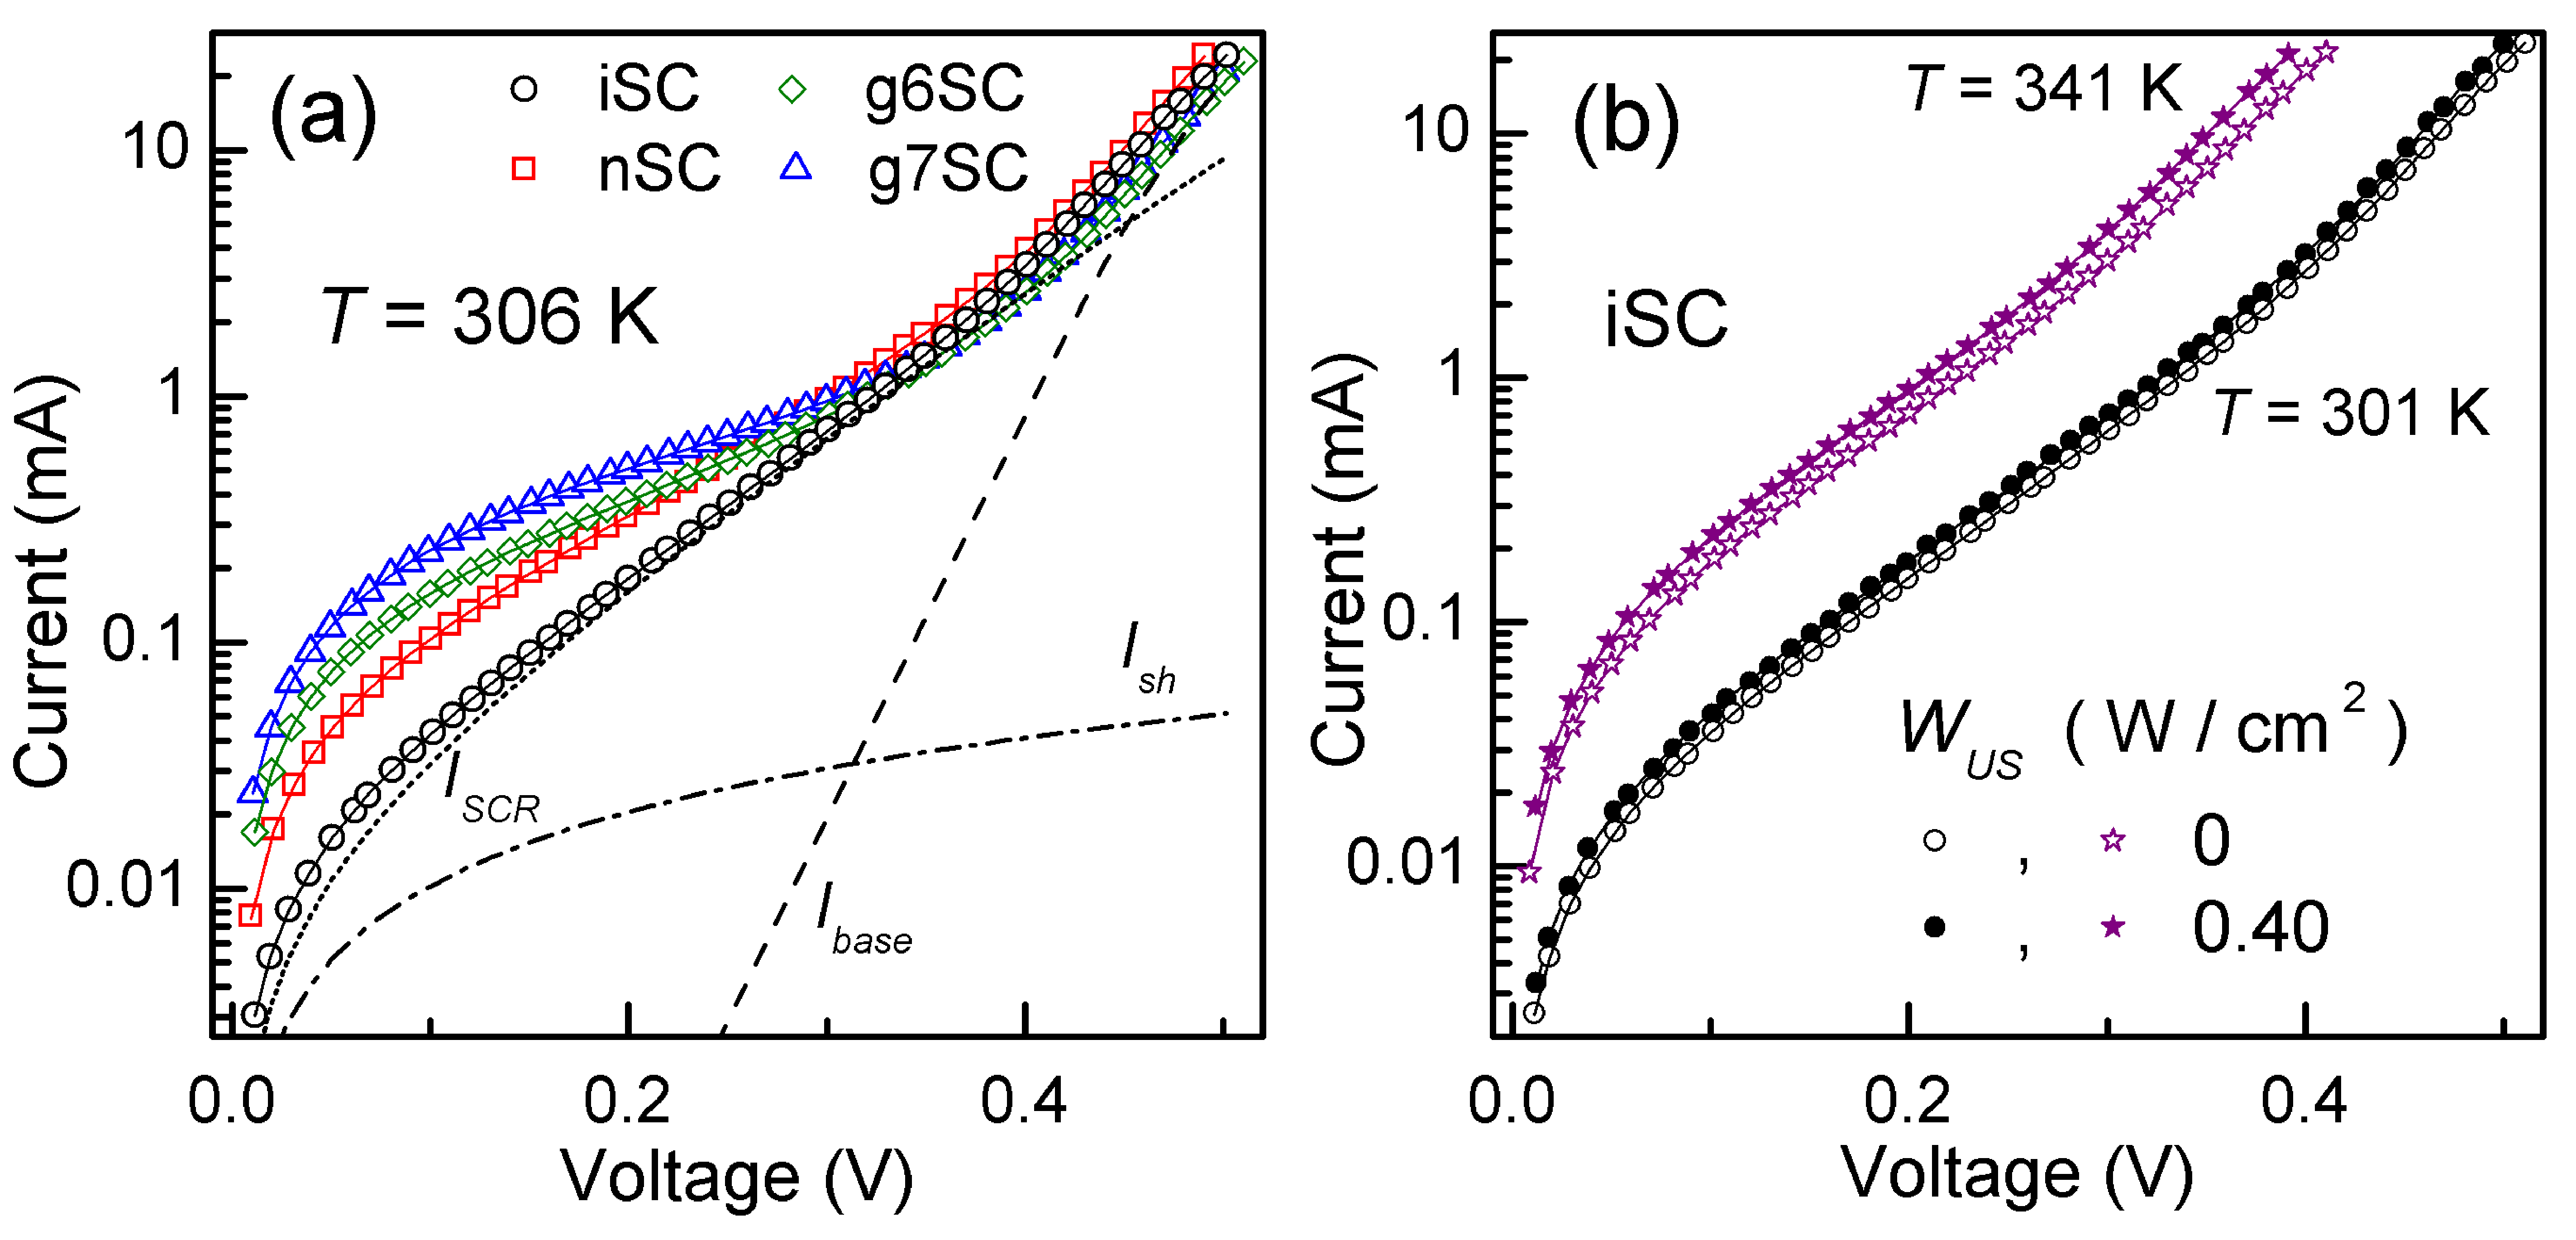
\includegraphics[width=0.7\textwidth]{fig_1ab}%
\caption{\label{figIV}
Dark $I$--$V$ characteristics measured (a) at 306~K for non--irradiated (circles), neutron--irradiated (squares) and gamma--irradiated (diamonds and triangles) structures without USL;
(b) at 301~K (circles) and 341~K (asterisks) with (filled marks, Ui--2) and without (open marks) USL for the iSC.
The marks are the experimental results, and the solid lines are the curves  fitted by Eqs.~(\ref{eqIV})--(\ref{eqW}).
The dashed, dotted and dotted--dashed lines in (a) represent the calculated base, SCR, and shunt components of total iSC current (black solid line).
}%
\end{figure*}


The double--diode model of n$^+$--p structure $I$--$V$ characteristics is expressed in the following form:
\begin{eqnarray}
I(V,T)&=&I_{SCR}+I_{base}+I_{sh}\;,\label{eqIV}\\
I_{SCR}&=&\frac{qAn_id}{2\tau_{g}}\left\{\exp \left[\frac{q(V-IR_s)}{n_{\mathrm{id}}kT}\right]-1\right\}\,,\label{eqIscr}\\
I_{base}&=&\frac{qAn_i^2}{p_p}\sqrt{\frac{\mu_nkT}{\tau_n}}\left\{\exp \left[\frac{q(V-IR_s)}{kT}\right]-1\right\},\label{eqIbase}\\
I_{sh}&=&(V-IR_s)/R_{sh}\,,\label{eqIsh}
\end{eqnarray}
where
$I_{SCR}$ describes the overall SCR recombination,
$I_{base}$ is closely related to the recombination in the quasi--neutral region,
$I_{sh}$ is the shunt current,
$A$ is the sample area,
$n_i$ is the intrinsic carrier concentration,
$\tau_{g}$ is the SCR carrier lifetime,
$d$ is the  SCR thickness:
\begin{equation}
\label{eqW}
    d=\sqrt{\frac{2 \varepsilon \varepsilon_0}{q p_p}\left[
     \frac{E_g}{q}-\frac{kT}{q}\ln\!\left(\frac{N_vN_c}{p_pn_n}\right)-\frac{2kT}{q}-V\right]},
\end{equation}
$\varepsilon$ is the permittivity (11.7 for Si),
$p_p$ and $n_n$ are the majority carrier concentration in $p$-- and $n$--type regions,
$E_g$ is the semiconductor band gap,
$N_c$ and $N_v$ are the effective densities of states in the conduction and valence bands;
$n_{\mathrm{id}}$ is the ideality factor,
$R_s$ and $R_{sh}$ are the series and shunt resistances,
and $\mu_n$ and $\tau_n$ are the mobility and lifetime of the electron (minority carrier) in the diode base.

We used Eqs. (\ref{eqIV})--(\ref{eqW}) to fit the experimental data taking $\tau_g$, $\tau_n$, $n_{\mathrm{id}}$, $R_{sh}$, and $R_s$ as the  fitting parameters.
Also, we used the known \cite{ni:Green,Schroder2006,Markvart} temperature dependences of $n_i$, $E_g$, and $\mu_n$.
As a result, we obtained extremely good fit to the experimental data --- see Fig.~\ref{figIV}.
In particular, for all the samples, the value of $R_s$ was found to be about 1~$\Omega$.
The broken lines in Fig.~\ref{figIV}(a) show an example of the calculated contributions of $I_{SCR}$, $I_{base}$, and $I_{sh}$ to the total current.

In case of USL, the transverse AWs with the frequency of $4.2$~MHz, which were exited by using piezoelectric transducer,  were applied to the samples at the base side in the [111]--direction.
The US intensities $W_{\mathtt{US}}$, amplitudes of lattice deformation $\xi_{\mathtt{US}}$, and lattice atom
displacements  $u_{\mathtt{US}}$ are listed in Table~\ref{tabUSL}.
It was reported previously \cite{Ostapenko1995,Olikh:Ultras,Ostrovskii2001} that the characteristic time of change in silicon structure parameters under
the US action  did not exceed $2\times10^3$~s.
In order to wait until the AI transitional period is competed, the following experimental procedure was used.
When USL started, the sample was first exposed to room temperature for 60~min and then the $I$--$V$ measurement and the sample heating were started.
In order to avoid the effect of piezoelectric field on $I$--$V$ characteristics, the piezoelectric transducer was shielded.

\begin{table}
\caption{\label{tabUSL}The ultrasound loading parameters.
}
\begin{ruledtabular}
\begin{tabular}{ccccc}
Sample&$W_{\mathtt{US}}$ (W/cm$^2$)&$\xi_{\mathtt{US}}$ ($10^{-6}$)&$u_{\mathtt{US}}$ (nm)&USL label\\
\hline
iSC&0.22&3.1&0.67&Ui--1\\
&0.40&4.2&0.91&Ui--2\\
nSC&0.24&3.2&0.70&Un--1\\
&0.40&4.2&0.91&Un--2\\
g6SC&0.38&4.1&0.89&Ug6--2\\
g7SC&0.19&2.9&0.63&Ug7--1\\
&0.37&4.0&0.87&Ug7--2\\
\end{tabular}
\end{ruledtabular}
\end{table}

Fig.~\ref{fig_Reverse} illustrates the reversibility of AI effects.
The time interval between USL initiation and "during" measurement was longer than 60~min,
and the time interval between USL termination and "after" measurement was about 24~h.
The data for nSC and g6SC are similar to those presented for iSC and g7SC.



\begin{figure*}
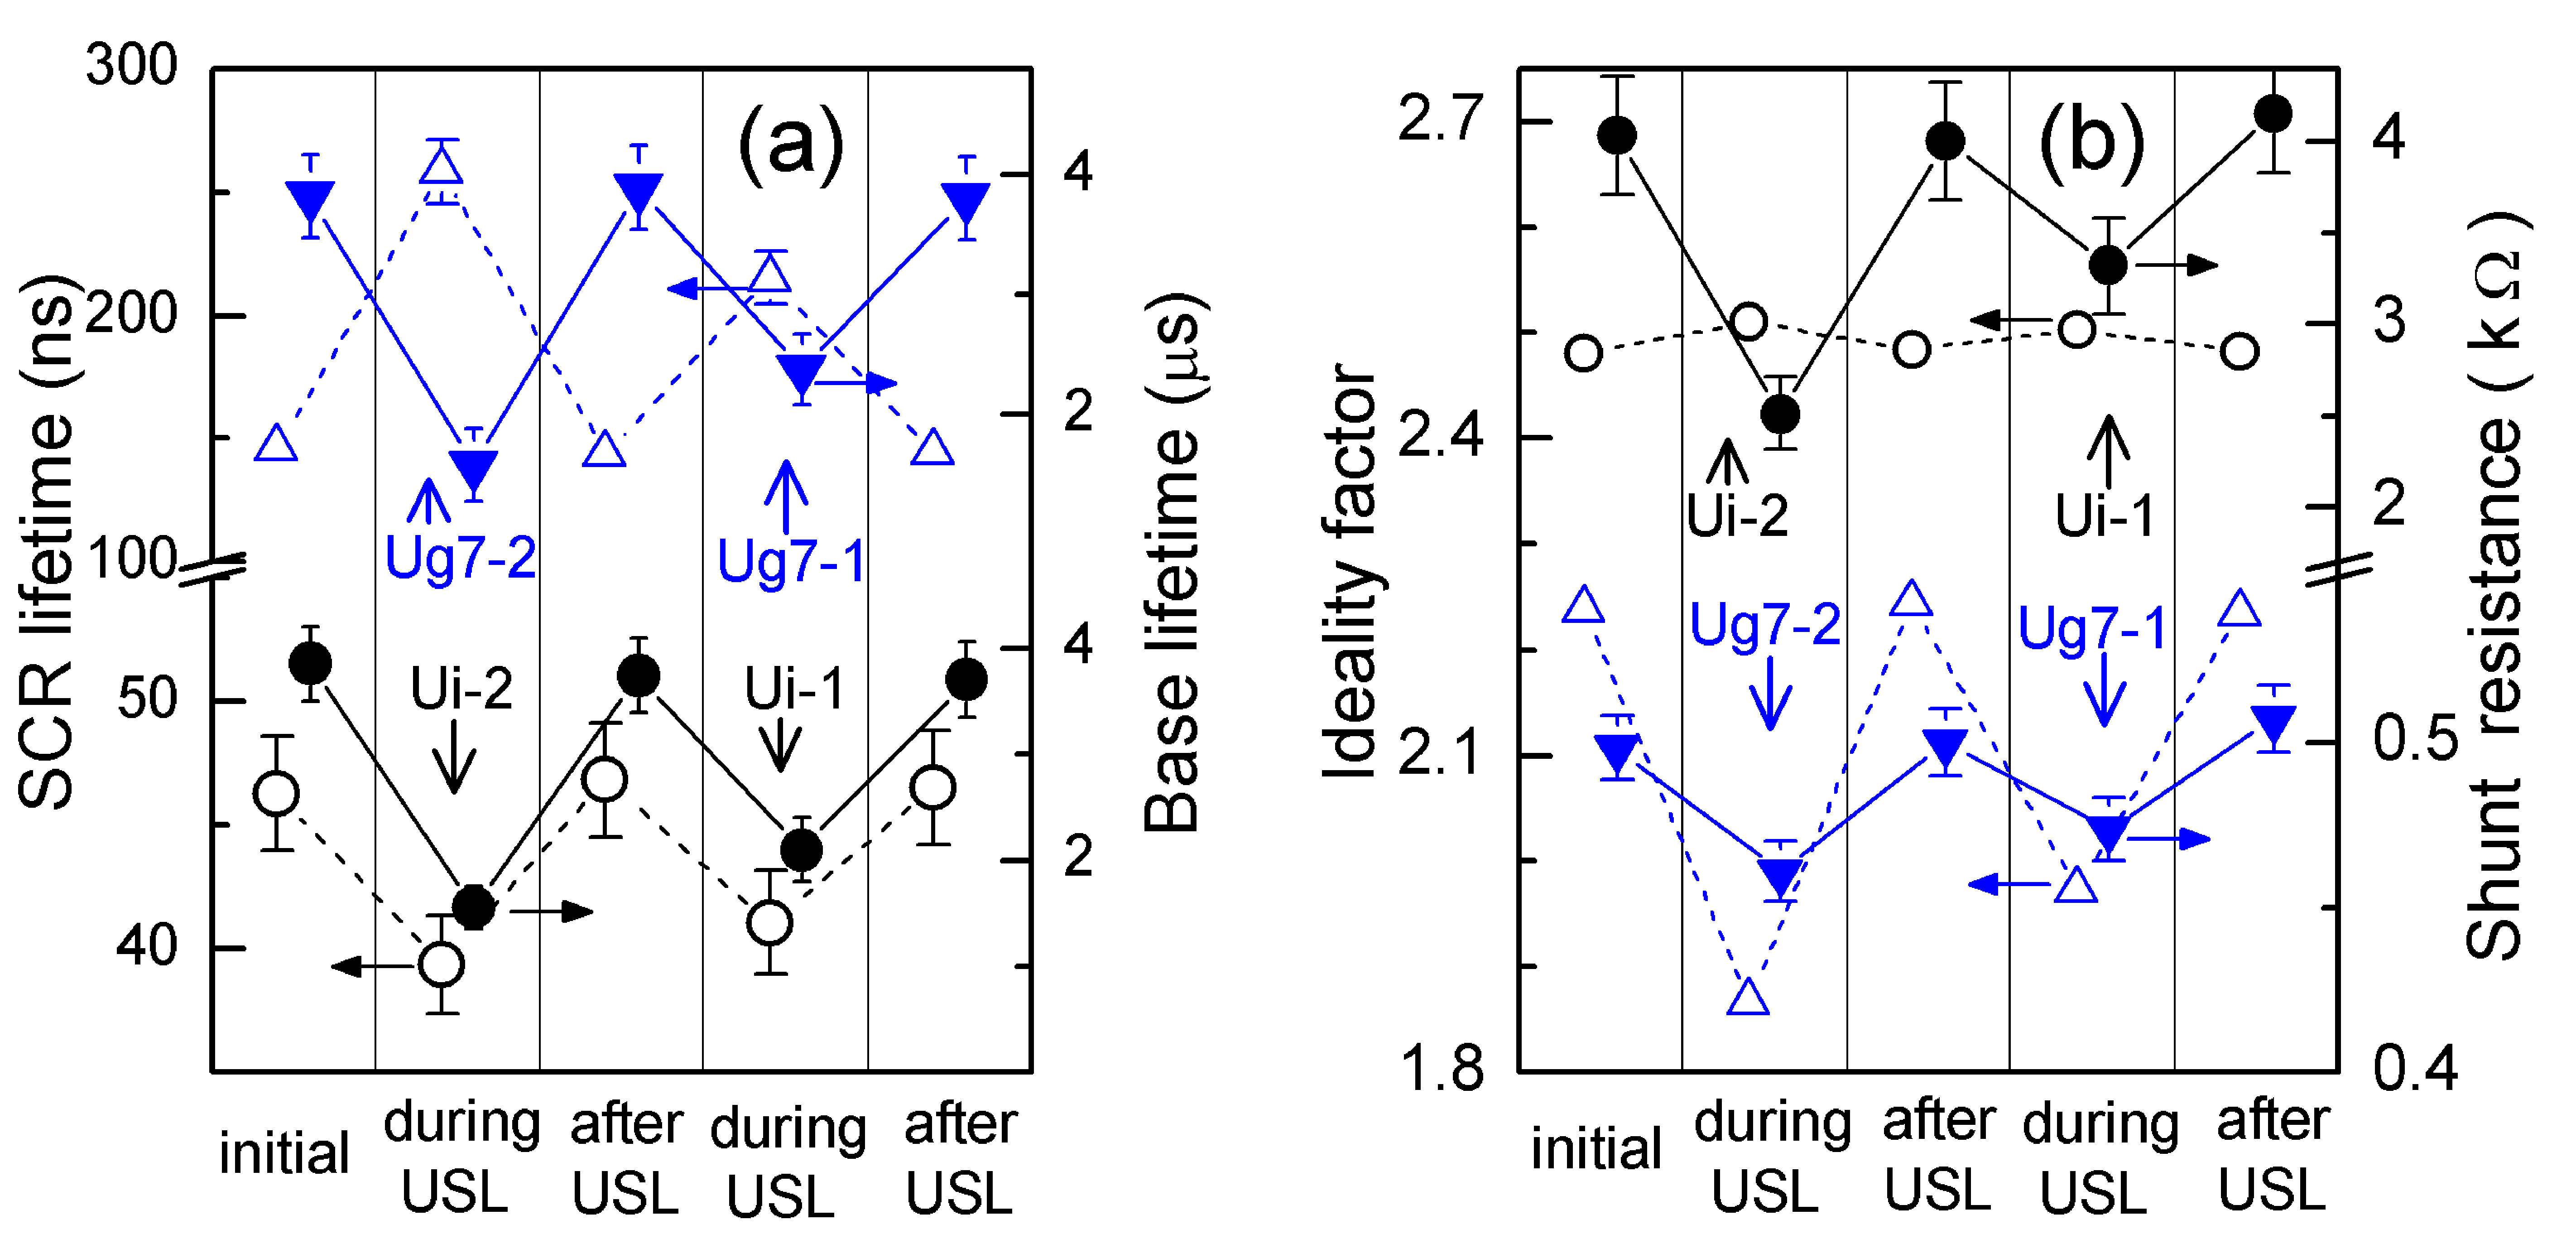
\includegraphics[width=0.7\textwidth]{fig_2ab}%
\caption{\label{fig_Reverse}
SCR lifetime (a, left axis, open marks),
base lifetime (a, right axis, filled marks),
ideality factor (b, left axis, open marks), and
shunt resistance (b, right axis, filled marks)
obtained before, during, and after USL at 330~K.
Data for iSC (circles) and g7SC (triangles) are presented.
}%
\end{figure*}


The non-linear fittings were performed by using the differential evolution method.\cite{DEWang}


\section{Results and Discussion}
\subsection{Space charge region\label{SCR}}
The parameters of $I$--$V$ characteristics associated with SCR phenomena are $n_{\mathrm{id}}$ and $\tau_{g}$.
The temperature dependences of the ideality factor and SCR carrier lifetime are shown in Fig.~\ref{fig_n} and Fig.~\ref{fig_TAUg}, respectively.

\begin{figure*}
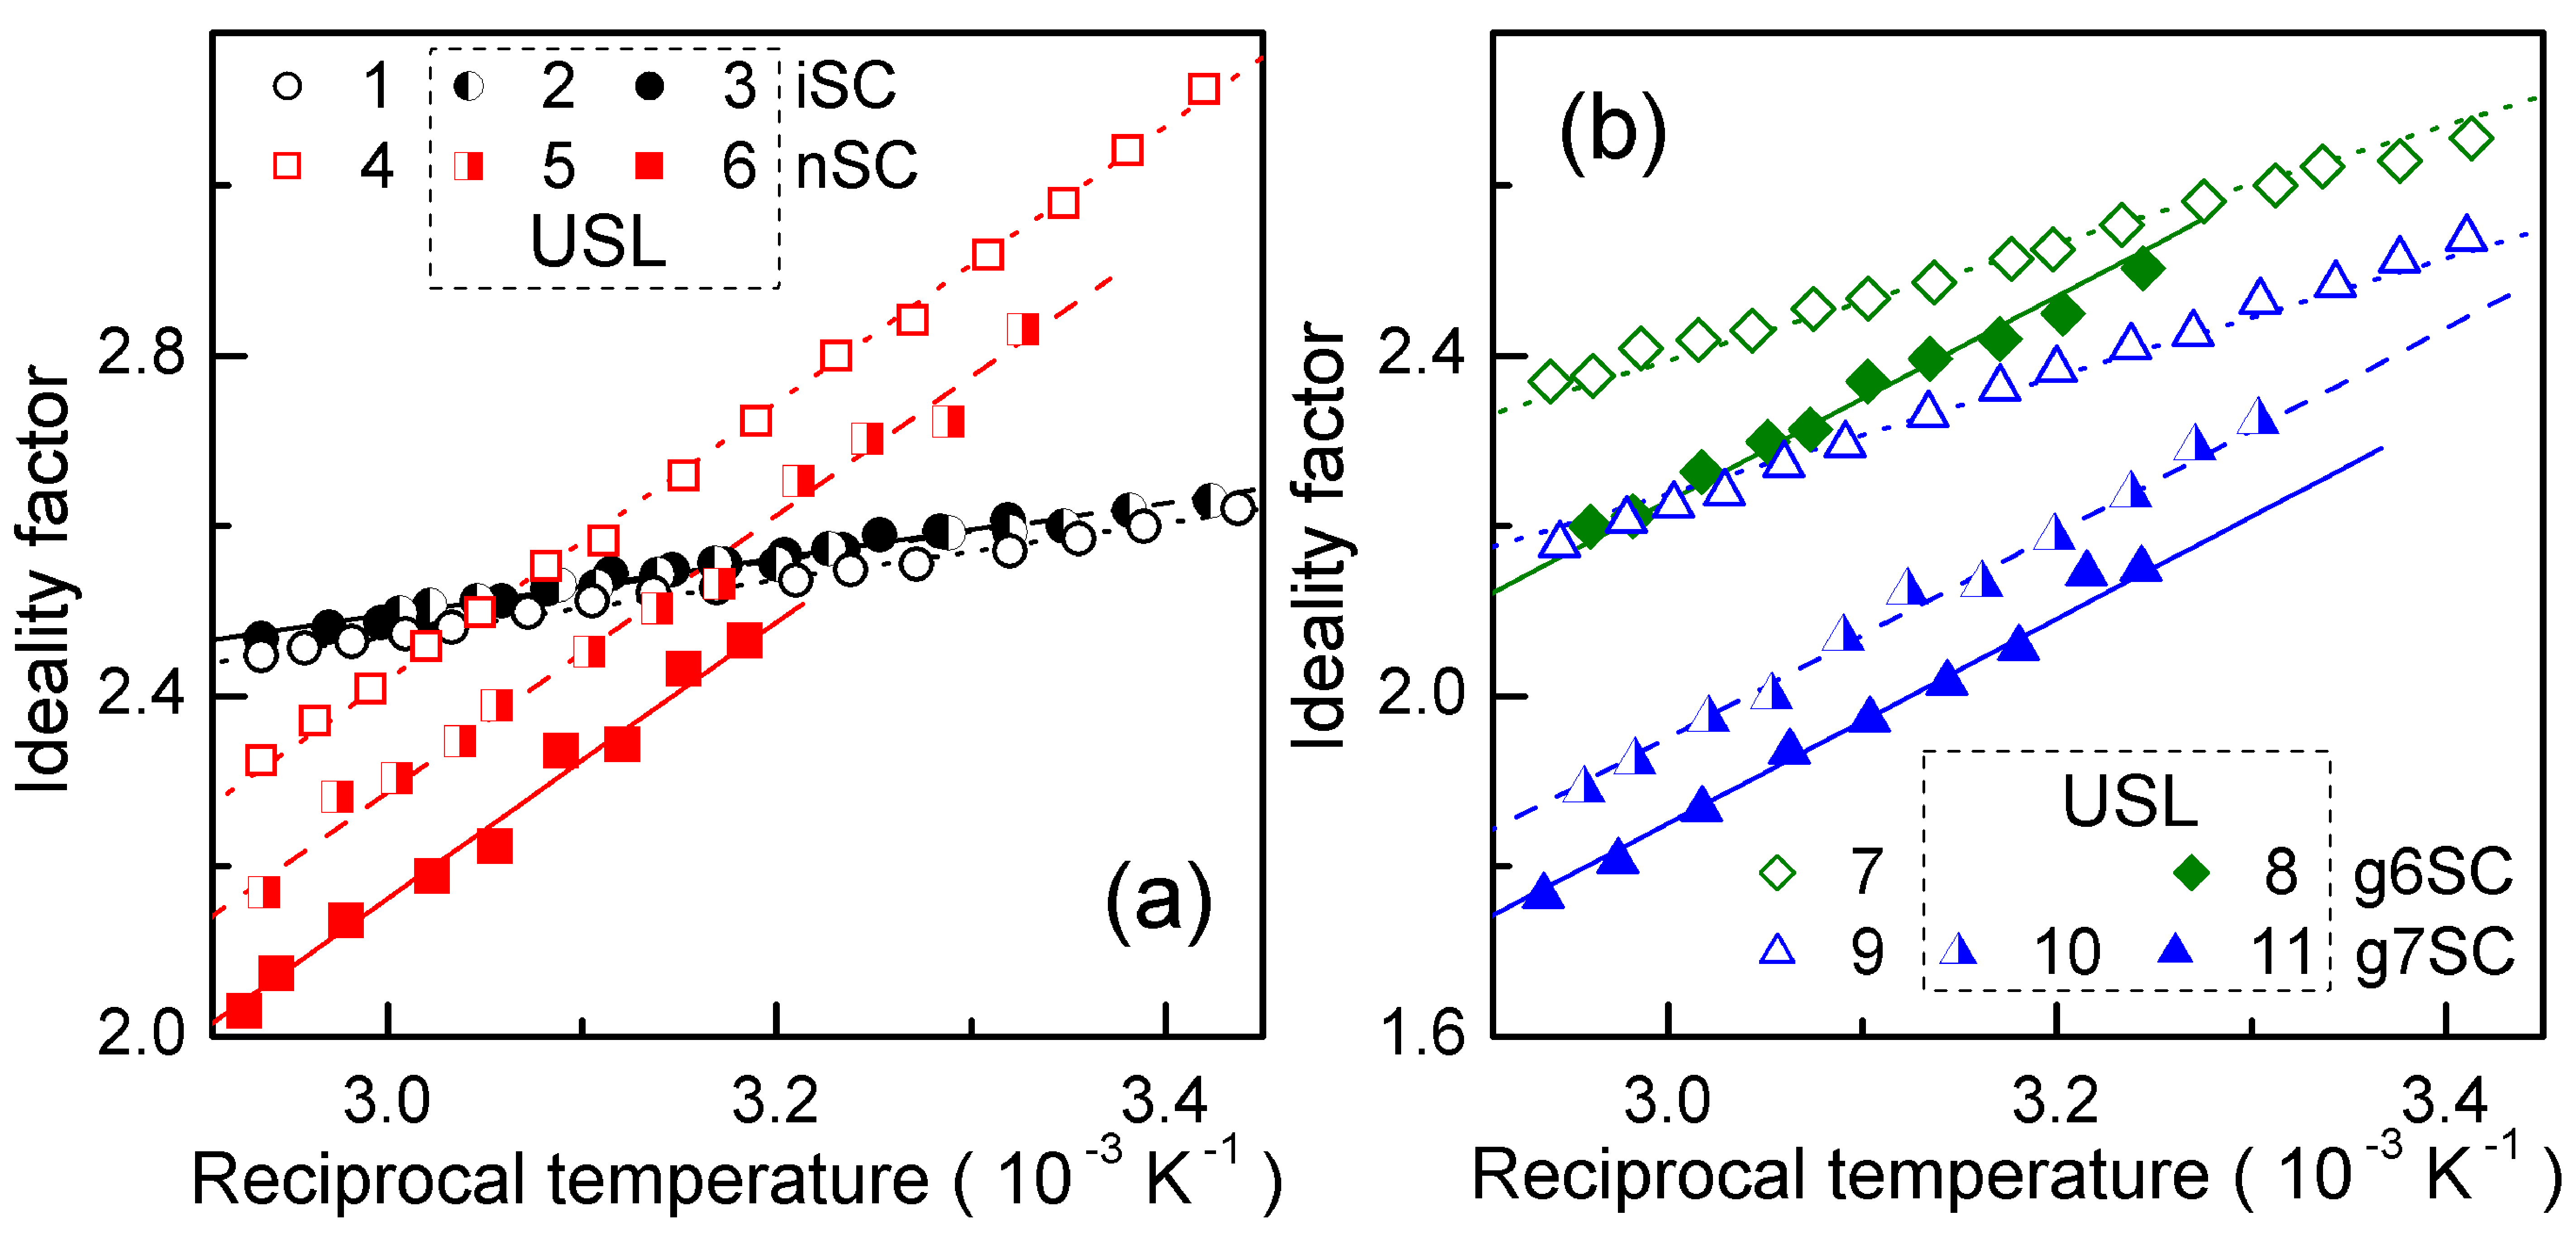
\includegraphics[width=0.7\textwidth]{fig_3ab}%
\caption{\label{fig_n}
Temperature dependences of the ideality factor for non--irradiated (curves 1--3, circles),
neutron--irradiated (4--6, squares), and $\gamma$--irradiated (7--11, diamonds and triangles) samples.
The curves 1, 4, 7, and 9 (open marks) are obtained without USL,
and curves 2, 3, 5, 6, 8, 10, and 11 correspond to
Ui--1, Ui--2, Un--1, Un--2, Ug6--2, Ug7--1, and Ug7--2 respectively.
The marks are the experimental results, and the lines are the fitted curves using Eq.~(\ref{eq_nT}).
}%
\end{figure*}

\begin{figure*}
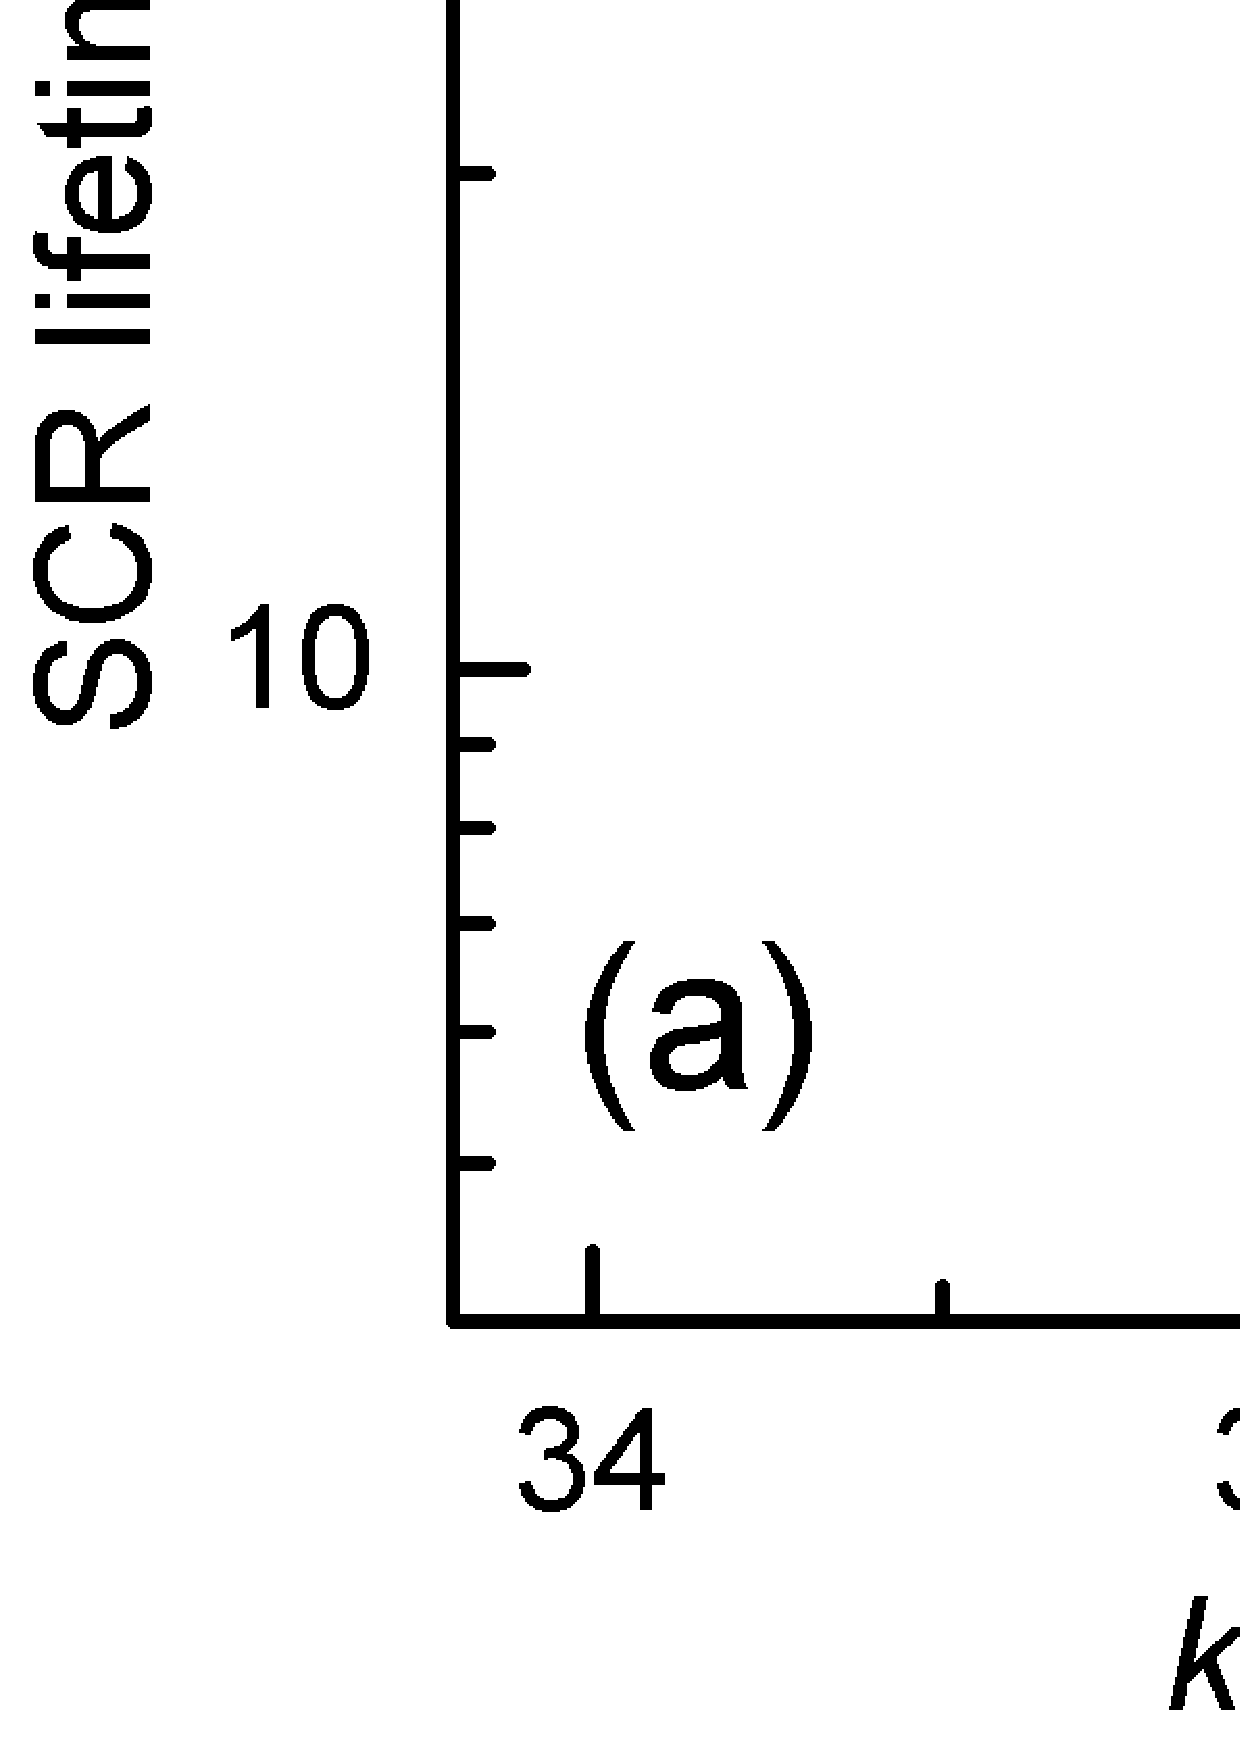
\includegraphics[width=0.7\textwidth]{fig_4ab}%
\caption{\label{fig_TAUg}
Temperature dependences of SCR lifetime for non--irradiated (curves 1--3, circles),
neutron--irradiated (4--6, squares), and $\gamma$--irradiated (7--11, diamonds and triangles) samples.
The curves 1, 4, 7, and 9 (open marks) are obtained without USL,
and curves 2, 3, 5, 6, 8, 10, and 11 correspond to
Ui--1, Ui--2, Un--1, Un--2, Ug6--2, Ug7--1, and Ug7--2 respectively.
The marks are the experimental results, and the lines are the fitted curves using Eq.~(\ref{eq_TAUgT}).
}%
\end{figure*}

As shown in Fig.~\ref{fig_n}, the ideality factor decreases with the increase in temperature, and the  dependence of $n_{\mathrm{id}}$ on $1/T$  is close to linear.
Thus, dependence $n_{\mathrm{id}}(T)$ can be expressed as
\begin{equation}
\label{eq_nT}
    n_{\mathrm{id}}(T)=n_{\mathrm{id},\infty}+T_{\mathrm{id}}/T\:.
\end{equation}
The thermoactivated growth of SCR lifetime is observed over the explored temperature range --- see Fig.~\ref{fig_TAUg}.
The temperature dependence of $\tau_{g}$ is well described by the following equation
\begin{equation}
\label{eq_TAUgT}
    \tau_{g}(T)=\tau_{g0}\exp\left(-\frac{E_{\tau g}}{kT}\right)\:.
\end{equation}
The values of $T_{\mathrm{id}}$ and $E_{\tau g}$ found for both non--irradiated and irradiated samples under USL as well as without USL are listed in Table~\ref{tabTpar}.


\begin{table*}
\caption{\label{tabTpar}Characteristics of temperature dependences of $n^+$--$p$--Si structure parameters.
}
\begin{ruledtabular}
\begin{tabular}{cccccc}
Sample&USL&$T_{\mathrm{id}}$ (K)&$E_{\tau g}$ (eV)&$R_{293,\mathtt{Al}}$ (k$\Omega$)&$\sigma_{\mathtt{dis}}$ ($10^4$~K/$\Omega$)\\
\hline
iSC&non&$330\pm30$&$0.24\pm0.01$&$27\pm3$&$41\pm4$\\
&Ui--1&$310\pm30$&$0.24\pm0.01$&$27\pm3$&$50\pm4$\\
&Ui--2&$360\pm30$&$0.24\pm0.01$&$26\pm3$&$58\pm4$\\
nSC&non&$1610\pm70$&$0.45\pm0.02$&$2.2\pm0.4$&$65\pm7$\\
&Un--1&$1600\pm70$&$0.44\pm0.02$&$2.3\pm0.4$&$95\pm10$\\
&Un--2&$1680\pm70$&$0.44\pm0.02$&$2.2\pm0.4$&$130\pm10$\\
g6SC&non&$610\pm40$&$0.28\pm0.01$&$0.7\pm0.1$&$19\pm2$\\
&Ug6--2&$1080\pm50$&$0.33\pm0.02$&$0.8\pm0.1$&$24\pm2$\\
g7SC&non&$770\pm50$&$0.29\pm0.01$&$0.41\pm0.06$&$26\pm3$\\
&Ug7--1&$1260\pm60$&$0.34\pm0.02$&$0.39\pm0.06$&$45\pm4$\\
&Ug7--2&$1270\pm60$&$0.35\pm0.02$&$0.38\pm0.06$&$55\pm4$\\
\end{tabular}
\end{ruledtabular}
\end{table*}

We would like to stress that

\noindent
(i)~irradiation leads to changes in $T_{\mathrm{id}}$ and $E_{\tau g}$ , and g6SC's characteristic temperature of the ideality factor and SCR lifetime characteristic energy are closely related to those of g7SC under similar conditions;

\noindent
(ii)~USL affects $n_{\mathrm{id}}$ and $\tau_g$ values;
the absolute AI changes of the ideality factor $\Delta n_{\mathrm{id}}=n_{\mathrm{id},\mathtt{US}}-n_{\mathrm{id},in}$ and
the relative AI changes of SCR lifetime $\varepsilon_{\tau g}=(\tau_{g,\mathtt{US}}-\tau_{g,in})/\tau_{g,in}$
(where subscripts ``$\mathtt{US}$'' and ``$in$'' indicate the values
obtained at the same temperature with and without USL, respectively)
are listed in Table~\ref{tabAIchange};

\noindent
(iii)~$\Delta n_{\mathrm{id}}$ and $\varepsilon_{\tau g}$ vary with $W_{\mathtt{US}}$ enhancement, whereas $T_{\mathrm{id}}$ and $E_{\tau g}$ values practically do not depend on US intensity;

\noindent
(iv)~USL leads to the increase  in both $T_{\mathrm{id}}$ and $E_{\tau g}$ in $\gamma$--irradiated samples [see Fig.~\ref{fig_n}(b) and Fig.~\ref{fig_TAUg}(b)],
but this effect is not observed in non--irradiated and neutron--irradiated samples [see Fig.~\ref{fig_n}(a) and Fig.~\ref{fig_TAUg}(a)];


\noindent
(v)~$\Delta n_{\mathrm{id}}$ and $\varepsilon_{\tau g}$ have opposite signs for non--irradiated and irradiated samples
(for SCg6 not in the whole temperature range);

\noindent
(vi)~ideality factor is varied by USL more effectively in the irradiated samples.


\begin{table}
\caption{\label{tabAIchange}Acoustically induced change of $n^+$-$p$--Si structure parameters (at 330~K).
}
\begin{ruledtabular}
\begin{tabular}{cccccc}
Sample&USL&$\Delta n_{\mathrm{id}}$ &$\varepsilon_{\tau g}$ &$\varepsilon_{\tau n}$ &$\varepsilon_{\sigma\mathtt{dis}}$ \\
&&\mbox{($\pm0.01$)}&($\pm5$\%)&($\pm0.2$)&($\pm10$\%)\\
\hline
iSC&Ui--1&0.02&-14&0.7&20\\
&Ui--2&0.03&-17&1.4&40\\
nSC&Un--1&-0.13&5&1.5&50\\
&Un--2&-0.26&13&3.0&100\\
g6SC&Ug6--2&-0.15&2&2.3&30\\
g7SC&Ug7--1&-0.26&49&0.9&70\\
&Ug7--2&-0.36&70&1.9&110\\
\end{tabular}
\end{ruledtabular}
\end{table}

For the purpose of our analysis, it is important to discuss the recombination mechanism in SCR of the investigated samples.
According to classical SRH theory, the ideality factor must be smaller than 2, and
$\tau_g$ temperature dependence is expected \cite{TAUg:Schroder,TAUg:Aharoni} to be described by the relation  $\tau_g\simeq2\,\tau_n\sqrt{\sigma_n/\sigma_p}\cosh\left[\left(E_t-E_i\right)/kT\right]$
(where $\sigma_n$, $\sigma_p$, and  $E_t$ are the electron and hole capture cross sections (CCSs) and the energy  level of  the  recombination  center,
and $E_i$  is the  intrinsic  energy level).
In our case, $n_{\mathrm{id}}$ is greater than 2, and $\tau_g$ increases with temperature.
Therefore, SRH theory cannot be applied in our case.
Several attempts to account for large $n_{\mathrm{id}}$ value have been made by using different models.\cite{Heide,Beier,Shah,Kaminski_n}
However, all the observed features of SCR recombination (large ideality factor, independence on light intensity, dependence on temperature
as well as short carrier lifetime) can be explained by the model of coupled defect level recombination (CDLR) \cite{CDLR:JAP1995,CDLR:JAP} only.
This mechanism provides a rapid  direct  charge  transfer  between  defect levels.
The phenomenon was first observed experimentally,\cite{DAPR:Chen1991,DAPR:Chen1994}  after which it was recruited to explain the process in semiconductor diodes. \cite{CDLR:JAP1995,CDLR:JAP,CDLR:SSP}

According to the CDLR model, the recombination is the result of carrier exchange between two defect levels and crystal bands.
In particular, it is supposed\cite{CDLR:JAP} that the recombination rate is dominant at the sites where acceptor--like defect is coupled with donor-like defect.
In a simplified case, when there is no carrier exchange between the donor level $E_t^{\mathtt{D}}$ and valence band,
as well as between the acceptor level $E_t^{\mathtt{A}}$ and conduction band,
the recombination rate $R$ can be expressed\cite{CDLR:JAP1995} as
\begin{eqnarray}
R&=&\frac{R_{12}-\sqrt{R_{12}^{\,2}-4\tau_{n}^{\mathtt{D}}\tau_{p}^{\mathtt{A}}(np-n_i^2)(1-\epsilon)}}{2\tau_{n}^{\mathtt{D}}\tau_{p}^{\mathtt{A}}(1-\epsilon)}\;,\label{eqR}\\
R_{12}&=&\frac{(n+n_{\mathtt{D}})(p+p_{\mathtt{A}})}{R_{\mathtt{DA}}}+
\tau_{n}^{\mathtt{D}}(p+p_{\mathtt{D}})+\tau_{p}^{\mathtt{A}}(n+n_{\mathtt{A}}),\label{eqR12}\\
\tau_{n}^{\mathtt{D}}&=&(N_{\mathtt{D}}\,\sigma_{n}^{\mathtt{D}}\,\upsilon_{\mathrm{th},n})^{-1},\,\,\,\,
\tau_{p}^{\mathtt{A}}=(N_{\mathtt{A}}\,\sigma_{p}^{\mathtt{A}}\,\upsilon_{\mathrm{th},p})^{-1},\label{eqTAU}
\end{eqnarray}
where
$R_{\mathtt{DA}}$ is the coupling parameter,
$N_{\mathtt{D}}$ and $N_{\mathtt{A}}$ are the densities of donor and acceptor--like defects,
$\sigma_{n}^{\mathtt{D}}$ and $\sigma_{p}^{\mathtt{A}}$ are the electron CCS of the donor and hole CCS of the acceptor,
$\upsilon_{\mathrm{th},n}$ and $\upsilon_{\mathrm{th},p}$ are the thermal electron and hole velocities,
$n_{\mathtt{D,A}}$, $p_{\,\mathtt{D,A}}$, and $\epsilon$ depend on $E_t^{\mathtt{D}}$, $E_t^{\mathtt{A}}$, and level degeneracy  factors.
Since $\tau_g\propto R^{-1}$, the last three values are expected to provide a thermoactivated behavior of SCR lifetime.
Unfortunately, the equation does not account for the functional relation between $I$--$V$ characteristics parameters and attributes of defects taking part in CDLR.


According to Steingrube \emph{et al}.\cite{CDLR:JAP},
CCS for defect in a pair differs from that for an isolated defect and depends on the distance $r$ between the donor and the acceptor:
\begin{equation}
\label{eqSigma}
\sigma_{n,p}^{\mathtt{D,A}}(r)=C_{n,p}^{\mathtt{D,A}}\,r^2\,,
\end{equation}
where $C_{n}^{\mathtt{D}}$ and $C_{p}^{\mathtt{A}}$ are the constant values.
$R_{\mathtt{DA}}$ is proportional to the overlap integral of the defect wave functions as well.
If both defects are characterized by the H--like radial--symmetric wave function and equal Bohr radius $a_0$,
the following expression can be used: \cite{CDLR:JAP}
\begin{equation}
\label{eqRda}
R_{\mathtt{DA}} (r) \propto N_{\mathtt{D}}N_{\mathtt{A}}\left[1+\frac{r}{a_0}+\frac{1}{3}\left(\frac{r}{a_0}\right)^2\right]
   e^{-r/a_0}\,.
\end{equation}

In our opinion, the observed reversible AI modifications of $n_{\mathrm{id}}$ and $\tau_g$ are induced by
donor--acceptor distance alteration in the samples under USL.
In fact, according to the data,\cite{MirzadeJAP2011,PeleshchakUJF2016} the force acting on a point defect during USL can be expressed as
\begin{equation}
\label{eqFd}
F_d=\chi\,\Delta\Omega_d\frac{\partial \xi(z,t)}{\partial z}\,,
\end{equation}
where
$\chi$ is the bulk elasticity modulus,
$\Delta\Omega_d$ is the crystal volume change per defect,
$\xi$ is the crystal lattice deformation,
and AW propagates along $z$ axis,
$\partial \xi(z,t)/\partial z\propto \xi_{\mathtt{US}}$.
For the interstitial atoms and substitutional impurities with ionic radius exceeding the ionic radius of matrix
atoms, $\Delta\Omega_d > 0$, whereas
for the vacancies and substitutional impurities whose ionic radius is smaller than that of matrix atoms, $\Delta\Omega_d < 0$.
Therefore, a point defect vibrates under USL, so oscillation amplitude and phase are determined by both the defect character and AW intensity.

\begin{figure}
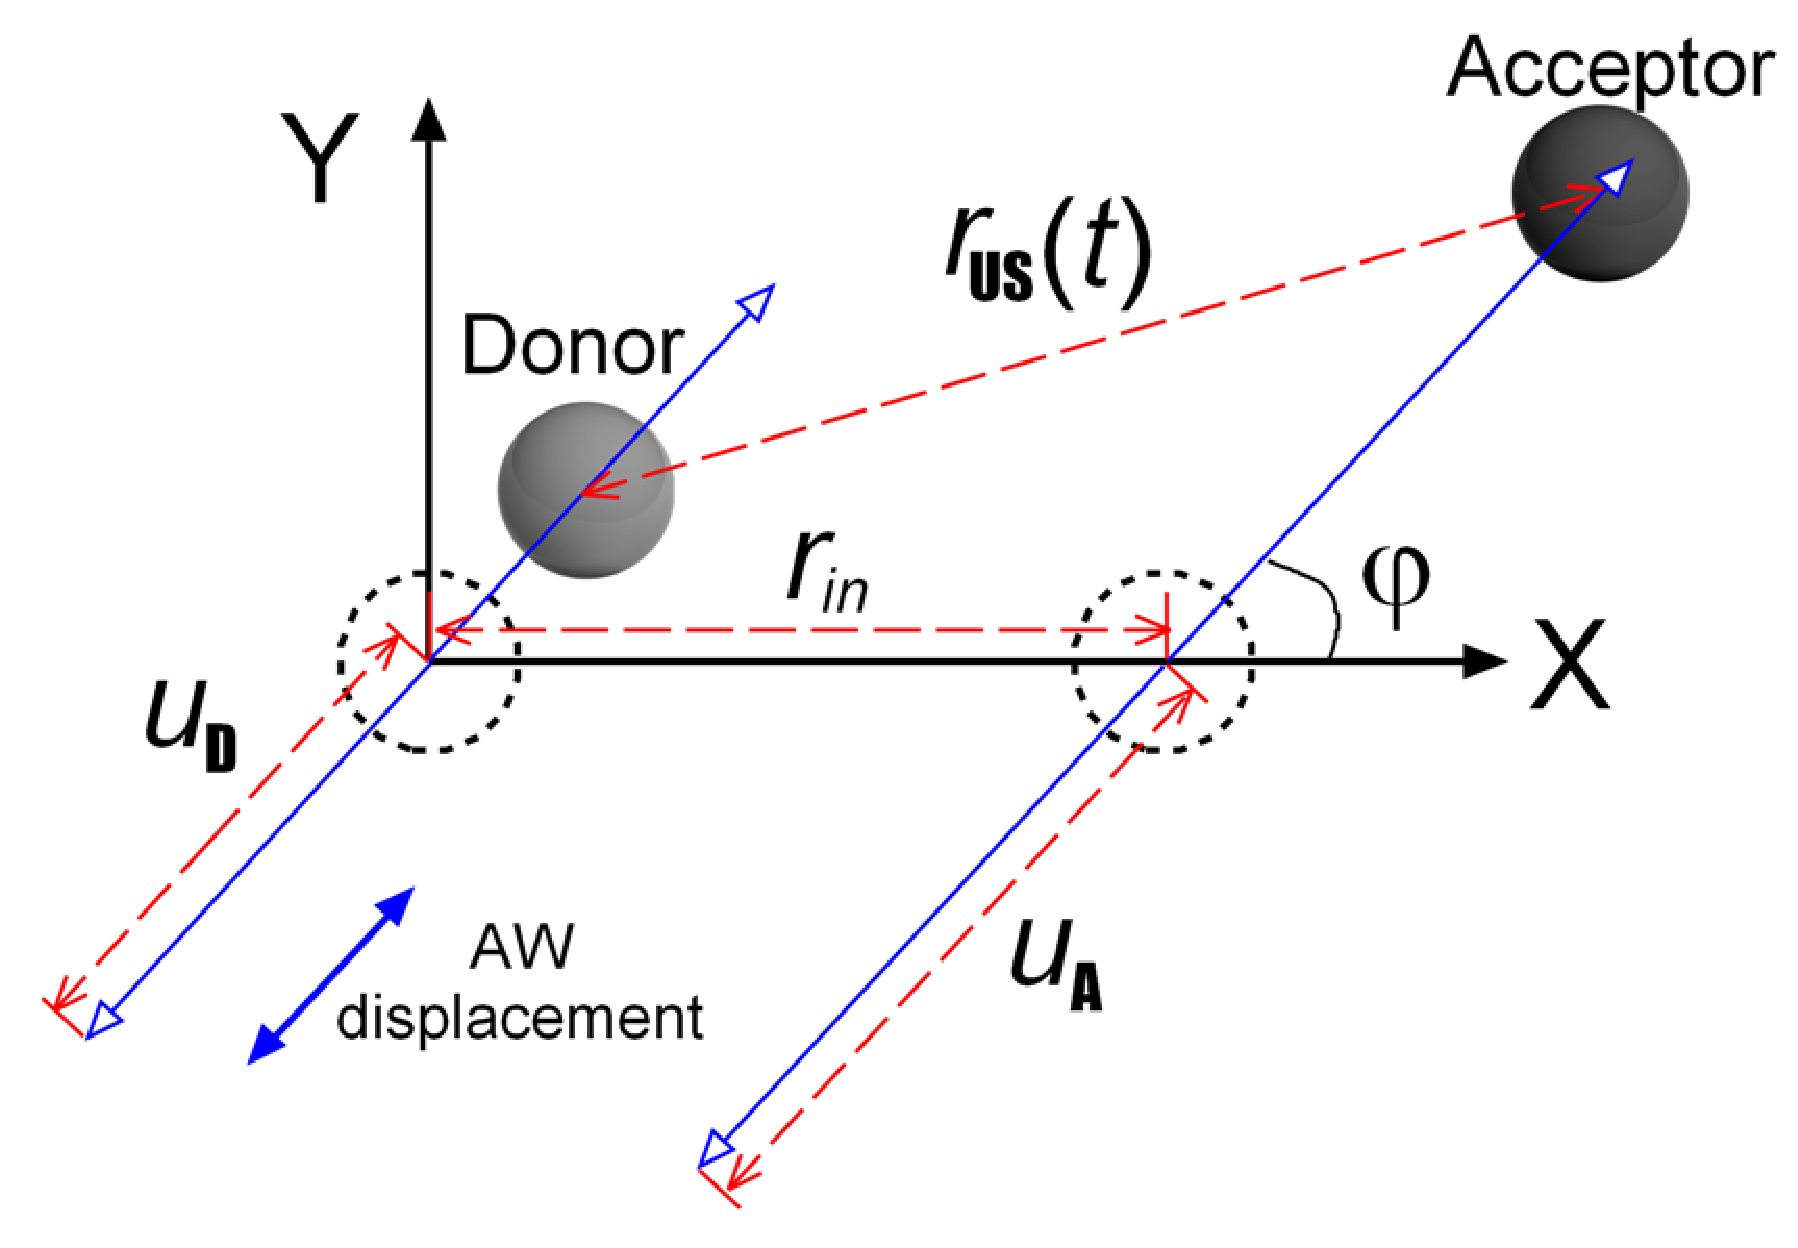
\includegraphics[width=0.45\textwidth]{fig_5}%
\caption{\label{fig_Model}
Model of CDLR center behavior under US action.
}%
\end{figure}


The simplest model, which is shown in Fig.~\ref{fig_Model}, gives the following  qualitative conclusion.
Initially, the donor and the acceptor are separated by the distance $r_{in}$,
and X axis is drawn through the point defect initial positions.
Under USL, the defects would vibrate with amplitudes $u_\mathtt{D}$ and $u_\mathtt{A}$.
The vibration axis coincides with AW displacement direction and forms angle $\varphi$ with  the X--axis.
Depending on $\xi_{U\!S}$, defect elastic strain ($\Delta\Omega_d^\mathtt{D}$ and $\Delta\Omega_d^\mathtt{A}$), and defect coupling the defect vibration amplitudes can have different values.
The donor--acceptor distance in the sample under USL $r_\mathtt{US}$, according to the model, depends on time $t$:
\begin{multline}
\label{eqrUS}
r_\mathtt{US}(t)=\left\{[r_{in}+u_\mathtt{A}\cos(\omega_\mathtt{US}t+\delta)-u_\mathtt{D}\cos(\omega_\mathtt{US}t)]^2\cos^2\varphi \right.\\
    \left.+ [u_\mathtt{A}\cos(\omega_\mathtt{US}t+\delta)-u_\mathtt{D}\cos(\omega_\mathtt{US}t)]^2\sin^2\varphi\right\}^{0.5}\,,
\end{multline}
where $\omega_\mathtt{US}$ is the US cyclic frequency and
$\delta$ is the phase shift between donor and acceptor vibration.

We use Eqs.~(\ref{eqSigma}) and (\ref{eqRda}) to estimate AI relative changes of CCS
$\varepsilon_\sigma=[\sigma_{\mathtt{US}}-\sigma(r_{in})]/\sigma(r_{in})$
and coupling parameters $\varepsilon_{\mathtt{RDA}}=[R_{\mathtt{DA,US}}-R_\mathtt{DA}(r_{in})]/R_\mathtt{DA}(r_{in})$,
where $\sigma_{\mathtt{US}}$ and $R_{\mathtt{DA,US}}$ are averaged over the AW period $T_\mathtt{US}$:
\begin{equation*}
\label{eqAver}
\sigma_{\mathtt{US}}=\frac{1}{T_\mathtt{US}}\int^{T_\mathtt{US}}_0\!\!\!\!\!\!\sigma(r_\mathtt{US}(t))dt\,,
R_{\mathtt{DA,US}}=\frac{1}{T_\mathtt{US}}\int^{T_\mathtt{US}}_0\!\!\!\!\!\!R_{\mathtt{DA}}(r_\mathtt{US}(t))dt\,.
\end{equation*}
In this estimation, the relaxation time in the CDLR sub--system is assumed to be considerably shorter than $T_\mathtt{US}$,
and we apply the previously used\cite{CDLR:JAP} value $a_0=3.23$~nm.
In addition, the chosen $u_\mathtt{D}$ and $u_\mathtt{A}$ values are commensurate with $u_\mathtt{US}$.
However, it should be taken into account that the displacement of the point defect without the covalent bond could exceed a matrix atom displacement.
Finally, no US  absorption by the defect is assumed.
In this simple case, $\delta$ is equal to $0^\circ$ if $(\Delta\Omega_d^\mathtt{D}\cdot\Delta\Omega_d^\mathtt{A})>0$
or to $180^\circ$ if $(\Delta\Omega_d^\mathtt{D}\cdot\Delta\Omega_d^\mathtt{A})<0$.
In addition, $\varepsilon_{\mathtt{RDA}}$ exclusively depends on
$|u_\mathtt{D}-u_\mathtt{A}|$ (in the $\delta=0^\circ$ case) or $|u_\mathtt{D}+u_\mathtt{A}|$ (in the $\delta=180^\circ$ case).
Moreover, these dependences are identical in both cases.
The typical results of simulation of coupling parameter changes are shown in  Fig.~\ref{fig_Erda}.

\begin{figure}
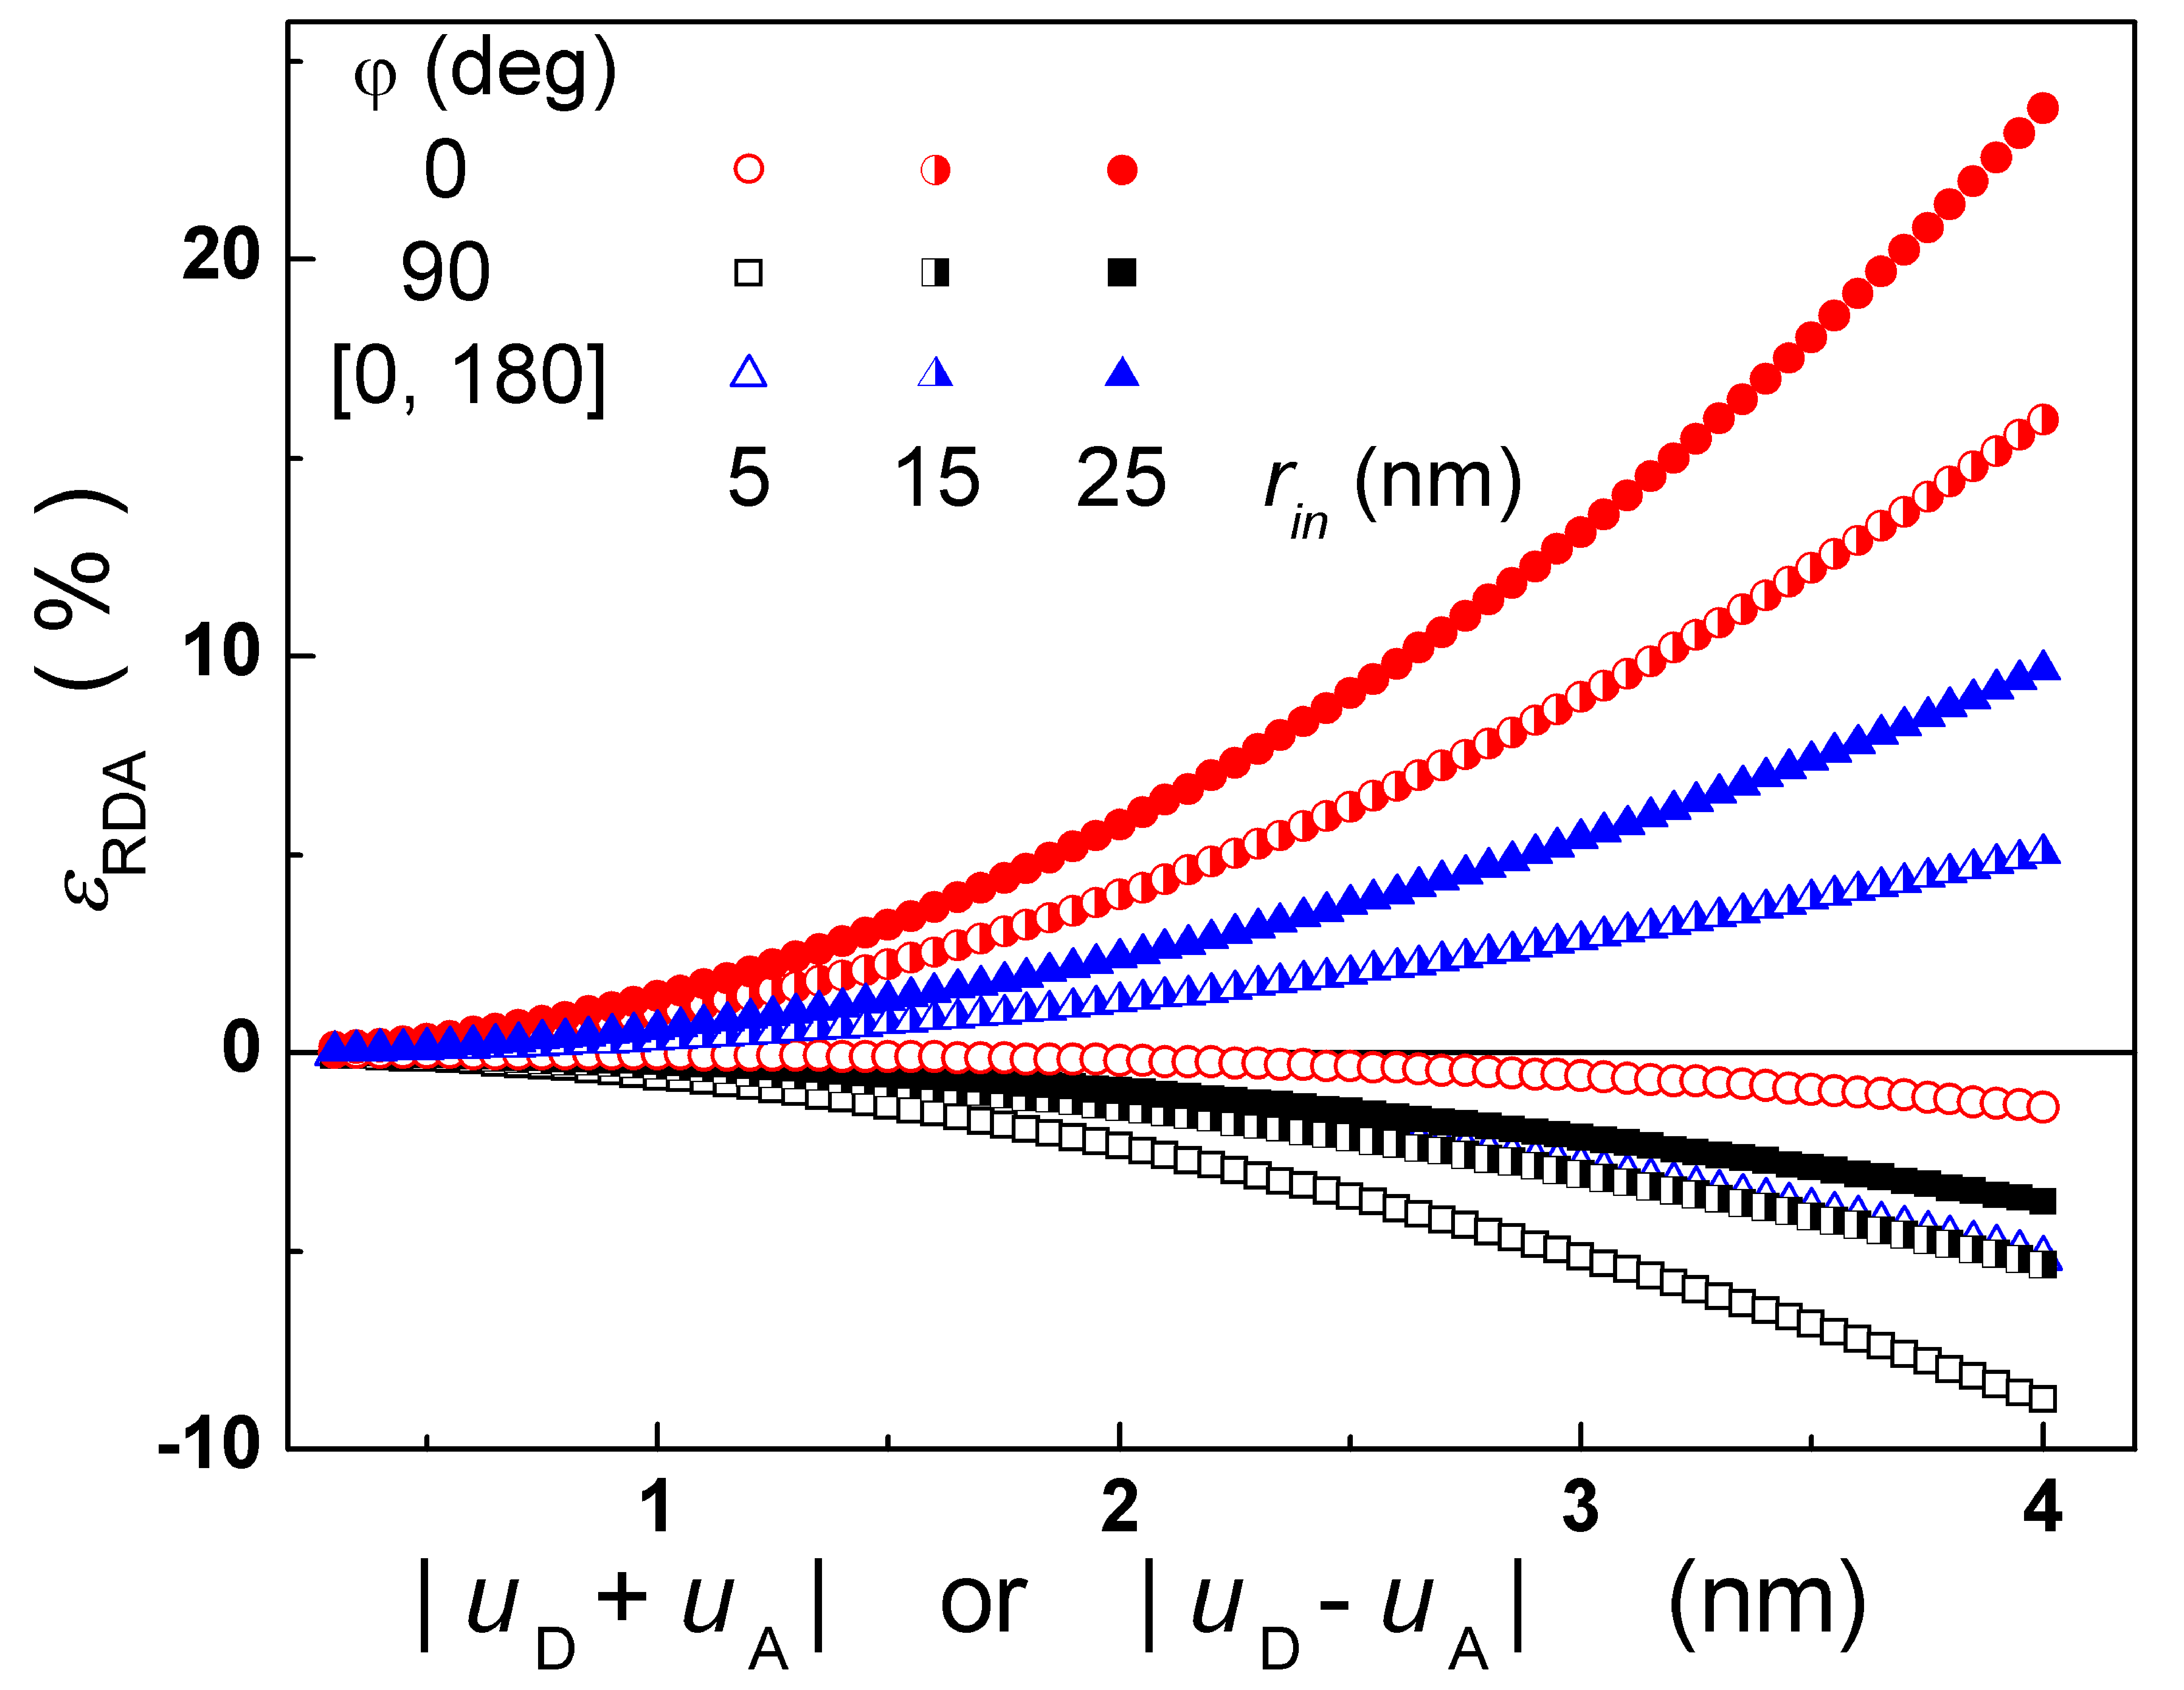
\includegraphics[width=0.45\textwidth]{fig_6}%
\caption{\label{fig_Erda}
Simulated dependencies of AI changes of coupling parameter on the vibration amplitudes.
Axis $|u_\mathtt{D}-u_\mathtt{A}|$ corresponds to $\delta=0^\circ$ case, whereas axis $|u_\mathtt{D}+u_\mathtt{A}|$ corresponds to $\delta=180^\circ$ case.
The parameters are set to $a_0=3.23$~nm,
$r_{in}=5$~nm (open marks), $15$~nm (semi--filled marks), and $25$~nm (filled marks),
$\varphi=0^\circ$ (circles), $90^\circ$ (squares).
Triangles correspond to mean $\varepsilon_{\mathtt{RDA}}$ value for $[0^\circ\div 180^\circ]$ $\varphi$ range.
}%
\end{figure}

Relative changes of CCS depend on oscillation amplitudes with similar features and
do not depend on $\varphi$:
\begin{equation}
\label{eqEpsSig}
\varepsilon_{\sigma}=(u_\mathtt{D}\pm u_\mathtt{A})^2/2\,r_{in}^2=K_\mathtt{US}^\mathtt{DA}W_{\mathtt{US}}\,,
\end{equation}
where``$+$'' and ``$-$'' correspond to $\delta=180^\circ$ and $\delta=0^\circ$, respectively,
$K_\mathtt{US}^\mathtt{DA}$ characterizes the defect couple--ultrasound interaction and depends on properties defects as well as crystal matrix.
Equation~(\ref{eqEpsSig}) takes into account that $u_\mathtt{D},u_\mathtt{A}\propto \xi_\mathtt{US}\propto\sqrt{W_\mathtt{US}}$.


It is worth keeping in mind that
CDLR current flows locally in the locations of extended defects.\cite{CDLR:JAP,CDLR:SSP}
At the same time, the dislocations are often located perpendicularly to the $p-n$ junction plane in the SCR region,
and the investigated samples are not exception (see Sec.~\ref{Rsh}).
If coupled defects and dislocations are close to each other, then the dislocations with the edge component should affect the pair spatial orientation.
Thus, the axis of donor--acceptor pair with $(\Delta\Omega_d^\mathtt{D}\cdot\Delta\Omega_d^\mathtt{A}>0)$  should be predominantly parallel to the dislocation line,
whereas the axis of a pair of coupled defects with $(\Delta\Omega_d^\mathtt{D}\cdot\Delta\Omega_d^\mathtt{A}<0)$ should make a right angle with the dislocation line.
As AW displacement is parallel to the $p-n$ junction plane,
the cases of most exciting interest are the following:

\noindent  $\delta=0^\circ$, $\varphi=90^\circ$ ($\Delta\Omega_d^\mathtt{D}\cdot\Delta\Omega_d^\mathtt{A}>0$ case);

\noindent  $\delta=180^\circ$, $\varphi\in[0^\circ\div 180^\circ]$ ($\Delta\Omega_d^\mathtt{D}\cdot\Delta\Omega_d^\mathtt{A}<0$ case).

\noindent
In other words, all curves in Fig.~\ref{fig_Erda} can be realized if defect volume relaxation of donor--like defect has the sign opposite to that of acceptor--like defect.
Moreover, only squares should to be under consideration in case of $\Delta\Omega_d^\mathtt{D}\cdot\Delta\Omega_d^\mathtt{A}>0$.

Taking into account the experimental results and the estimation obtained from our model:

\noindent
(i)~$E_{\tau g}$ and $T_{\mathrm{id}}$ are mainly determined by couple component energy levels.
The alteration of $E_{\tau g}$ and $T_{\mathrm{id}}$ for nSC, g6SC, and g7SC in comparison with iSC testifies to the change of defect (donor, acceptor, or both)
which take part in CDLR after irradiation.
g6SC defects are coincident to g7SC defects and differ from neutron--irradiated sample defect.

\noindent
(ii)~USL causes the donor--acceptor distance change and results in $\varepsilon_{\sigma}$ and $\varepsilon_{\mathtt{RDA}}$,
which increase with $W_{\mathtt{US}}$.

\noindent
(iii)~Acoustically induced $E_{\tau g}$ (and $T_{\mathrm{id}}$) modification, which is observed in g6SC and g7SC only,
testifies to the rebuilding of  $\gamma$--induced RD,
i.e., $\gamma$--induced RD is configurationally bistable (or metastable) and transforms from the ground state under US action.
Similar AI defect variations were also reported previously.\cite{Wosinski,Ostapenko1994,Olikh2009Sem,YOlikhTPL2011}

\noindent
(iv)~$\varepsilon_{\sigma}$ sign is immutable --- see Eq.~(\ref{eqEpsSig}),
whereas $\varepsilon_{\mathtt{RDA}}$ sign can vary for the pair with opposite relaxation volume component (see Fig.~\ref{fig_Erda}).
Therefore, the change of $\Delta n_{\mathrm{id}}$ and $\varepsilon_{\tau g}$ sign is the evidence of transformation
from $(\Delta\Omega_d^\mathtt{D}\cdot\Delta\Omega_d^\mathtt{A}>0)$  to
$(\Delta\Omega_d^\mathtt{D}\cdot\Delta\Omega_d^\mathtt{A}<0)$  after irradiation.
The transformation is confirmed by the enhanced efficiency of US action on defects in irradiated samples.
In fact, in the case of $(\Delta\Omega_d^\mathtt{D}\cdot\Delta\Omega_d^\mathtt{A}<0)$, the US efficiency is determined by the sum of pair component displacements,
whereas in the contrary case, it is determined by their difference.
In our opinion, both the donor and the acceptor are defects of interstitial--type in the non--irradiated sample, and one of pair components is a defect of vacancy--type in irradiated samples.
The defect configurations are discussed below, in Sec.~\ref{DefectType}.


\subsection{Quasi--neutral region\label{Base}}

Base lifetime describes the processes which occur in the quasi--neutral region  of the $p$-$n$ structure.
Fig.~\ref{fig_TAUr} shows  $\tau_n$  behaviour in the explored temperature range.
As expected, minority carrier lifetime increases as the temperature increases, and at 320~K,
$\tau_n$ values comprise  2-5~$\mu$s for different samples, which
correspond to 80-130~$\mu$m range of diffusion lengths.
In our opinion, the observed $\tau_n$ dispersion is caused not by irradiation but rather deals with sample--ancestor wafer inhomogeneity, which is often the case.\cite{Oxide:Chen,Oxide_Schon}

\begin{figure*}
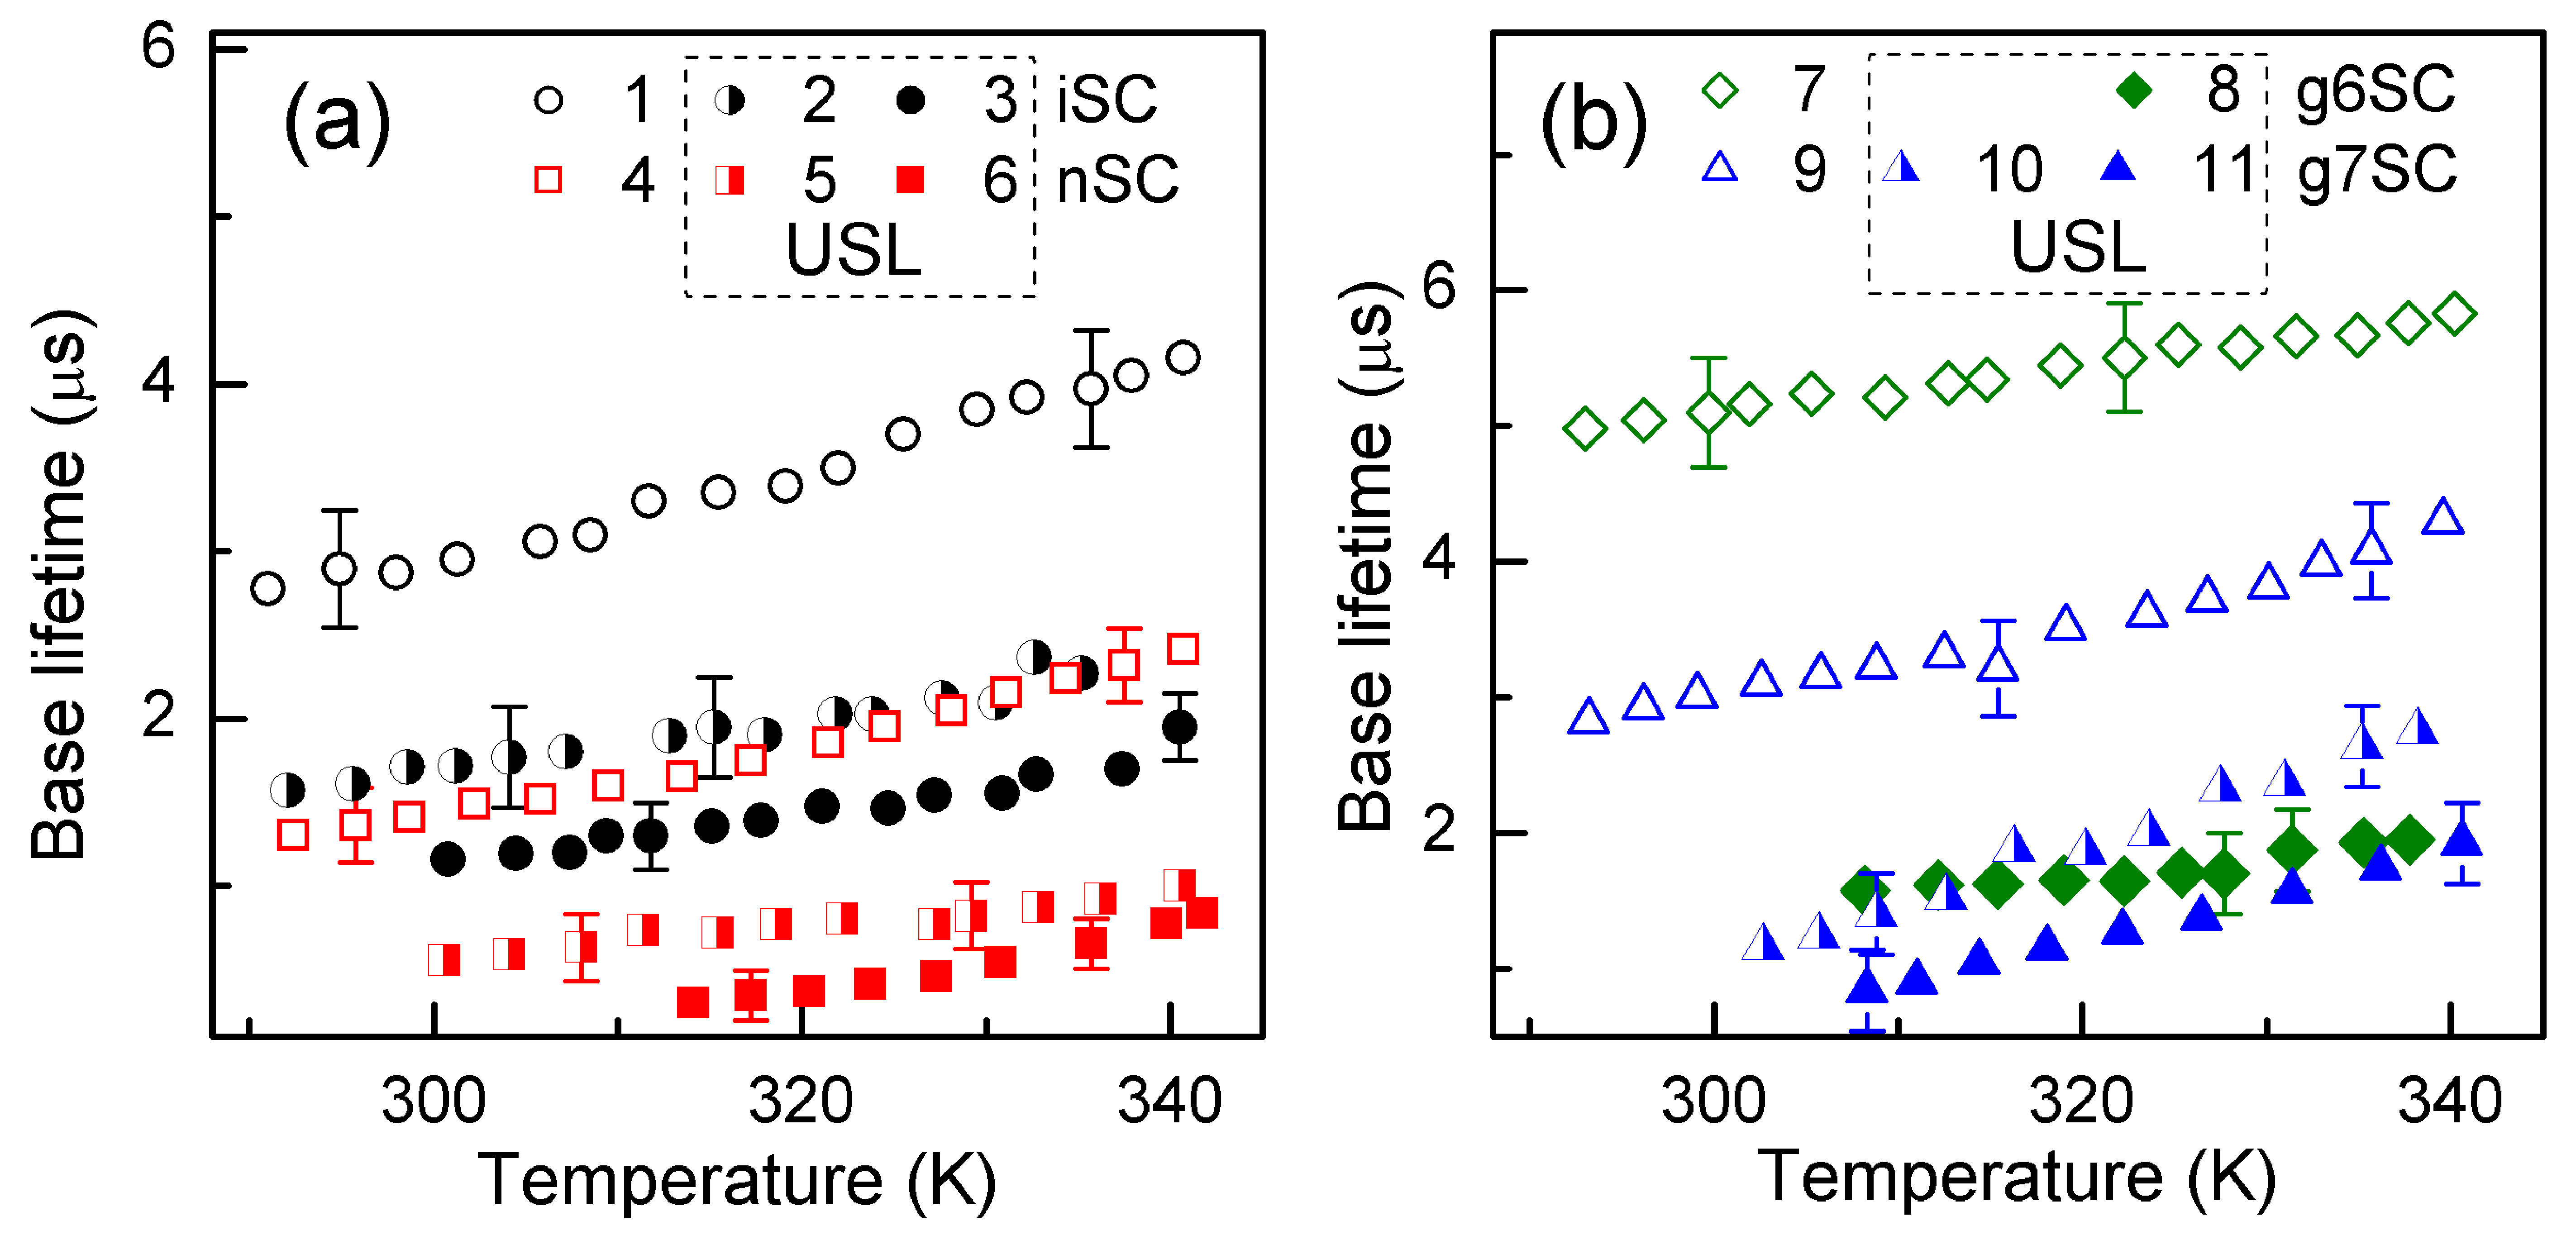
\includegraphics[width=0.7\textwidth]{fig_7ab}%
\caption{\label{fig_TAUr}
Temperature dependences of base lifetime for non--irradiated (curves 1--3, circles),
neutron--irradiated (4--6, squares), and $\gamma$--irradiated (7--11, diamonds and triangles) samples.
The curves 1, 4, 7, and 9 (open marks) are obtained without USL,
and curves 2, 3, 5, 6, 8, 10, and 11 correspond to
Ui--1, Ui--2, Un--1, Un--2, Ug6--2, Ug7--1, and Ug7--2, respectively.
}%
\end{figure*}

In fact,  the irradiation induced lifetime reduction is described by the Messenger–-Spratt equation:\cite{Markvart}
\begin{equation}
\label{eqMS}
\tau_n^{-1}=\tau_{n0}^{-1}+K_\tau\Psi\,,
\end{equation}
where $\tau_{n0}$ is the minority carrier lifetime in the non--irradiated sample
and $K_\tau$ is a lifetime damage constant.
The known $K_\tau$ values and estimated changes of reciprocal base lifetime $K_\tau\Psi$ are shown in Table~\ref{tabTAUn}.
As seen from the table, the estimated value of radiation--induced $\tau_n^{-1}$ change comprises (8-17), 4, and 29\% of
the values measured for samples nSC, g6SC, and g7SC, respectively, so this cannot explain the dispersion observed experimentally.
At the same time, the calculated lifetime changes $K_\tau\Psi$ are in quite good agreement with the changes expected from RDs production --- see Sec.~\ref{DefectType}.


\begin{table}
\caption{\label{tabTAUn}Measured and estimated base lifetime parameters.
}
\begin{ruledtabular}
\begin{tabular}{ccccc}
Sample &$\tau_{n,in}^{-1}$ (320~K)&$K_\tau$&$K_\tau\times\Psi$ &$K_\mathtt{US}^\mathtt{eff}$ \\
\hline
&(10$^5$~s$^{-1}$)&(cm$^2/$s)& (10$^4$~s$^{-1}$)&(cm$^2/$W) \\
iSC&2.9&$\ldots$&$\ldots$&3.5\\
nSC&4.7&10$^{-7}$(Ref.~\onlinecite{NIEL:Jafari})&\multirow{2}{*}{4$\div$8}&7.1\\
&&2$\times$10$^{-7}$(Ref.~\onlinecite{n:Gaubas})&&\\
g6SC&1.8&5$\times$10$^{-12}$&0.8&6.0\\
g7SC&2.8&(Refs.~\onlinecite{NIEL:Jafari} and \onlinecite{gamma:Kolkov})&8&5.2\\
\end{tabular}
\end{ruledtabular}
\end{table}

Base lifetime can be expressed as follows:\cite{MurphyJAP2011}
\begin{equation}
\label{eqTAUsum}
\tau_n^{-1}=\tau_\mathtt{bb}^{-1}+\tau_\mathtt{CE\,Auger}^{-1}+\tau_\mathtt{SRH}^{-1}\,,
\end{equation}
where
$\tau_\mathtt{bb}$, $\tau_\mathtt{CE\,Auger}$, $\tau_\mathtt{SRH}$ are the lifetimes of band--to--band recombination, Coloumb--enhanced Auger recombination, and
SRH recombination, respectively.
The calculation shows that $\tau_\mathtt{bb}^{-1}=14$~s$^{-1}$, $\tau_\mathtt{CE\,Auger}^{-1}=6$~s$^{-1}$.
Therefore, band--to--band recombination and Auger recombination can be neglected.
In case of the low injection level and single recombination centre, SRH lifetime is described by Eq.~(\ref{eqTAU}).
If there are  several centers of recombination, the following equation should be applied
\begin{equation}
\label{eqTAUSHRsum}
\tau_n^{-1}=\sum_i^{M_d}\tau_{n,i}^{-1}=\sum_i^{M_d}N_{d,i}\,\sigma_{n,i}\,\upsilon_{\mathrm{th},n}\,,
\end{equation}
where
$M_d$ is the total number of centers,
$\tau_{n,i}$ characterizes lifetime due to recombination by $i$--th defect,
and $N_{d,i}$ and $\sigma_{n,i}$ are the concentration and electron CCS of $i$--th defect, respectively.

Fig.~\ref{fig_TAUr} shows that USL results in a decrease in $\tau_n$.
Relative AI changes of reciprocal base lifetime $\varepsilon_{\tau n}=(\tau_{n,in}-\tau_{n,\mathtt{US}})/\tau_{n,\mathtt{US}}$
are listed in Table~\ref{tabAIchange}.
As AI changes are reversible, the lifetime alteration, in our opinion, deals with the increase in $\sigma_n$ under US action.
Following the empirical relation  proposed by Ref.~\onlinecite{CDLR:R2}, we assume that Eq.~(\ref{eqSigma})
is valid for a complex point defect as well.
In this case, however, $r$ is the distance which separates the components of a complex.
According to the model suggested in Sec.~\ref{SCR}, USL leads to $r$ variation
and $\sigma_n$ change in line with Eq.~(\ref{eqEpsSig}).
In the case of CDLR, AI change of the capture cross section of donor (or/and acceptor) is supplemental to the variation of
both the coupling parameter and the couple distance,
but only CCS change determines the AI variation of base lifetime.

However, not every defect effectively takes part in AID.
If  $M_d^\mathtt{AA}$ and $M_d^\mathtt{nonAA}$ are the total numbers of acoustically active (AA) and non--acoustically active (non--AA) centers,
Eq.~(\ref{eqTAUSHRsum}) for $\tau_{n}^{-1}$ under USL and without it takes the following shape:
\begin{eqnarray}
\tau_{n,in}^{-1}&=&\sum_j^{M_d^\mathtt{AA}}N_{d,j}\,\sigma_{n,j}^{in}\,\upsilon_{\mathrm{th},n}+
\sum_l^{M_d^\mathtt{nonAA}}N_{d,l}\,\sigma_{n,l}\,\upsilon_{\mathrm{th},n}\,,\nonumber\\
\tau_{n,\mathtt{US}}^{-1}&=&\sum_j^{M_d^\mathtt{AA}}N_{d,j}\,\sigma_{n,j}^\mathtt{US}\,\upsilon_{\mathrm{th},n}+
\sum_l^{M_d^\mathtt{nonAA}}N_{d,l}\,\sigma_{n,l}\,\upsilon_{\mathrm{th},n}\,.\nonumber
\end{eqnarray}
By using Eq.~(\ref{eqEpsSig}), $\varepsilon_{\tau n}$  is transformed as follows
\begin{equation}
\label{eqEpsTAU}
\varepsilon_{\tau n}=K_\mathtt{US}^\mathtt{eff}W_\mathtt{US}\,,
\end{equation}
where $K_\mathtt{US}^\mathtt{eff}$ characterizes ADI in the sample
and depends on the concentration of both AA and non--AA centers
\begin{equation}
\label{eqKeff}
K_\mathtt{US}^\mathtt{eff}=\sum_j^{M_d^\mathtt{AA}}\frac{\tau_{n,in}}{\tau_{n,j,in}}K_\mathtt{US,j}\,.
\end{equation}
Here, $K_\mathtt{US,j}$ deals with the $j$--th defect--ultrasound interaction.

The obtained dependences of $\varepsilon_{\tau n}$ vs $W_\mathtt{US}$ are shown in Fig.~\ref{fig_Kus}.
The linearity of these dependences proves the correctness of our assumptions.
The obtained $K_\mathtt{US}^\mathtt{eff}$ values are listed in Table~\ref{tabTAUn}.
The non--monotonic $K_\mathtt{US}^\mathtt{eff}$ alteration with $\gamma$ dose
is discussed in Sec.~\ref{DefectType}.

\begin{figure}
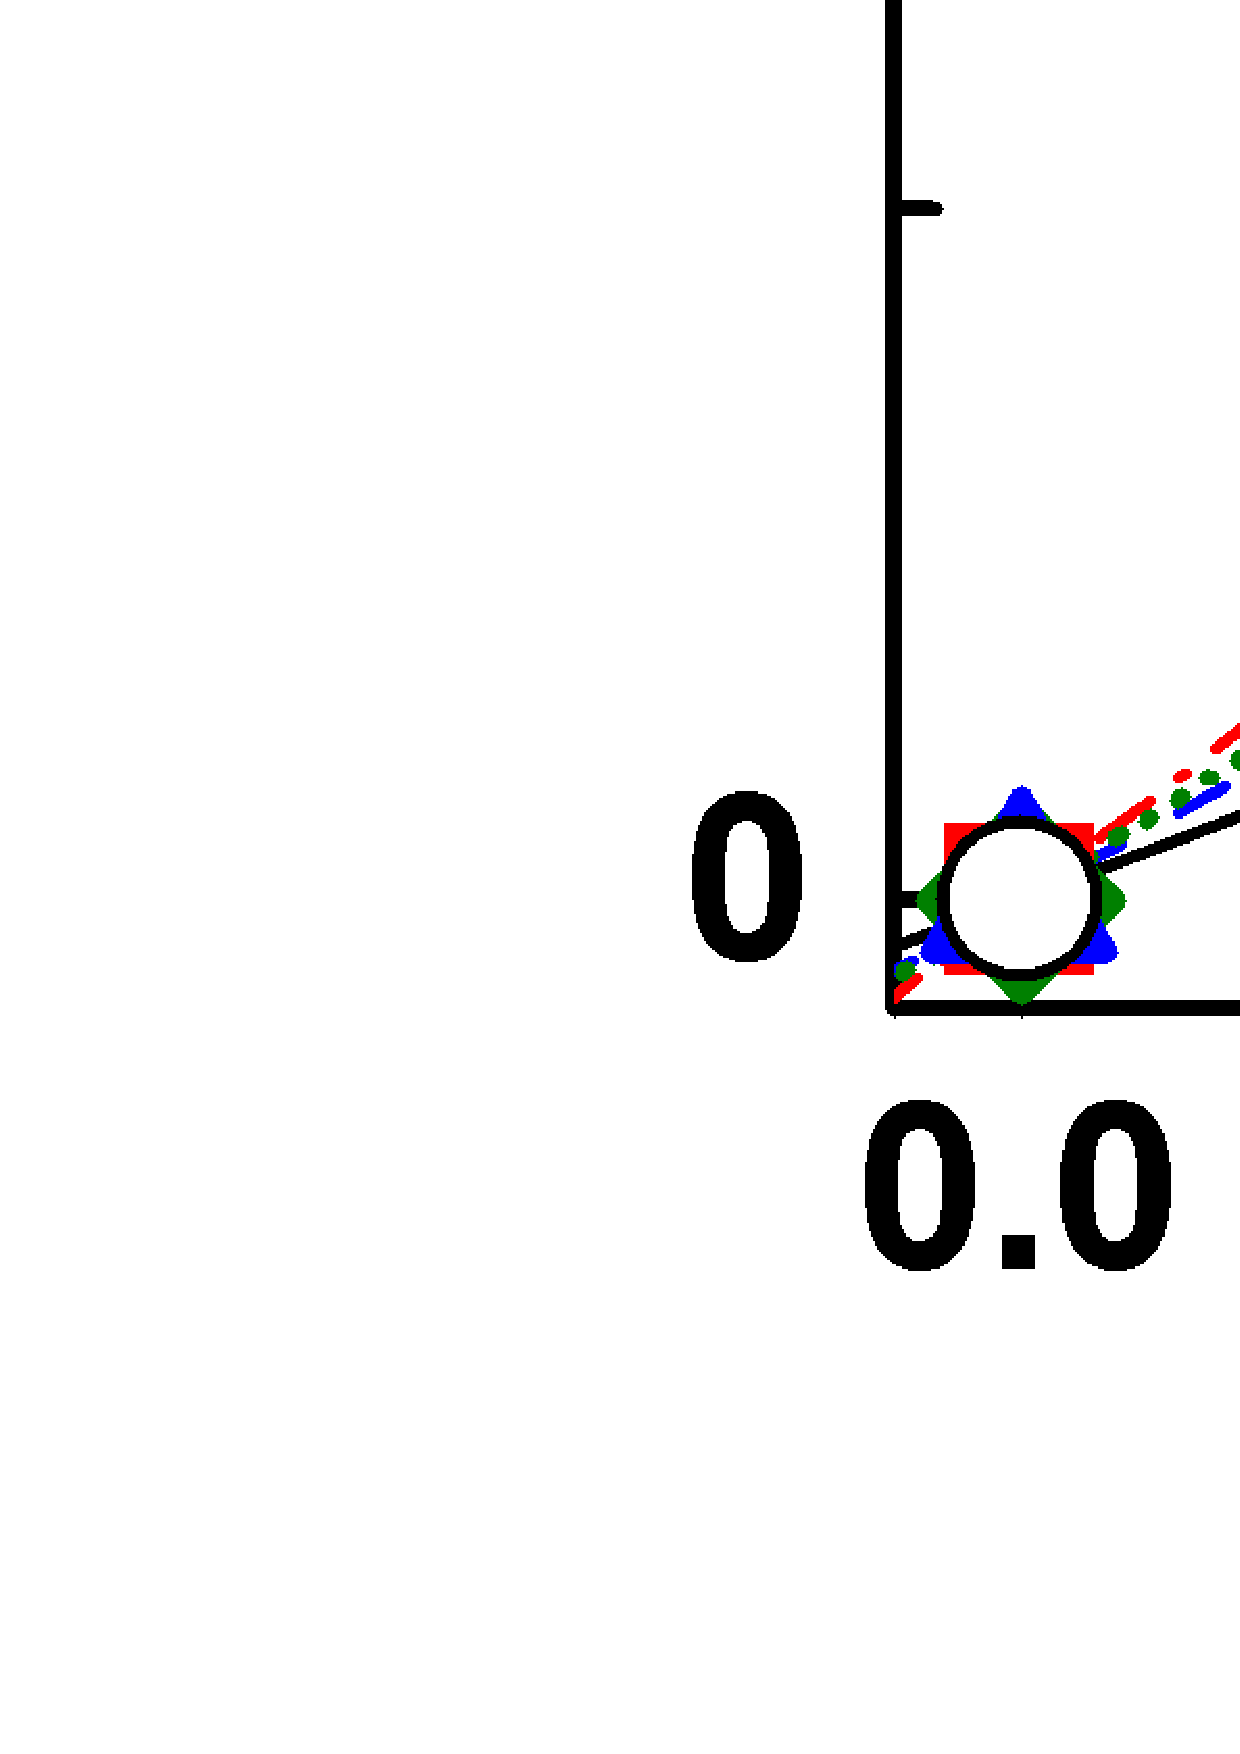
\includegraphics[width=0.45\textwidth]{fig_8}%
\caption{\label{fig_Kus}
Dependences of base lifetime relative change on US intensity for non--irradiated (circles), neutron--irradiated (squares), and $\gamma$--irradiated
(triangles and diamonds) samples.
Lines are the fitted curves using Eq.~(\ref{eqEpsTAU}).
}%
\end{figure}

\subsection{Shunt resistance\label{Rsh}}
Fig.~\ref{fig_Rsh} shows the  shunt resistance  over the explored temperature range.
As seen from the figure, the irradiation results in a decrease in $R_{sh}$.
Also, the $R_{sh}$ temperature dependence changes after $\gamma$ irradiation.
In particular,  the shunt resistance decreases with the temperature growth in iSC and nSC,
whereas in g6SC and g7SC, the increase in $R_{sh}$ vs $T$  is close to linear in the vicinity of 293~K.
It should be noted that $R_{sh}$ axis is logarithmic in Fig.~\ref{fig_Rsh}(a) and linear in Fig.~\ref{fig_Rsh}(b).


\begin{figure*}
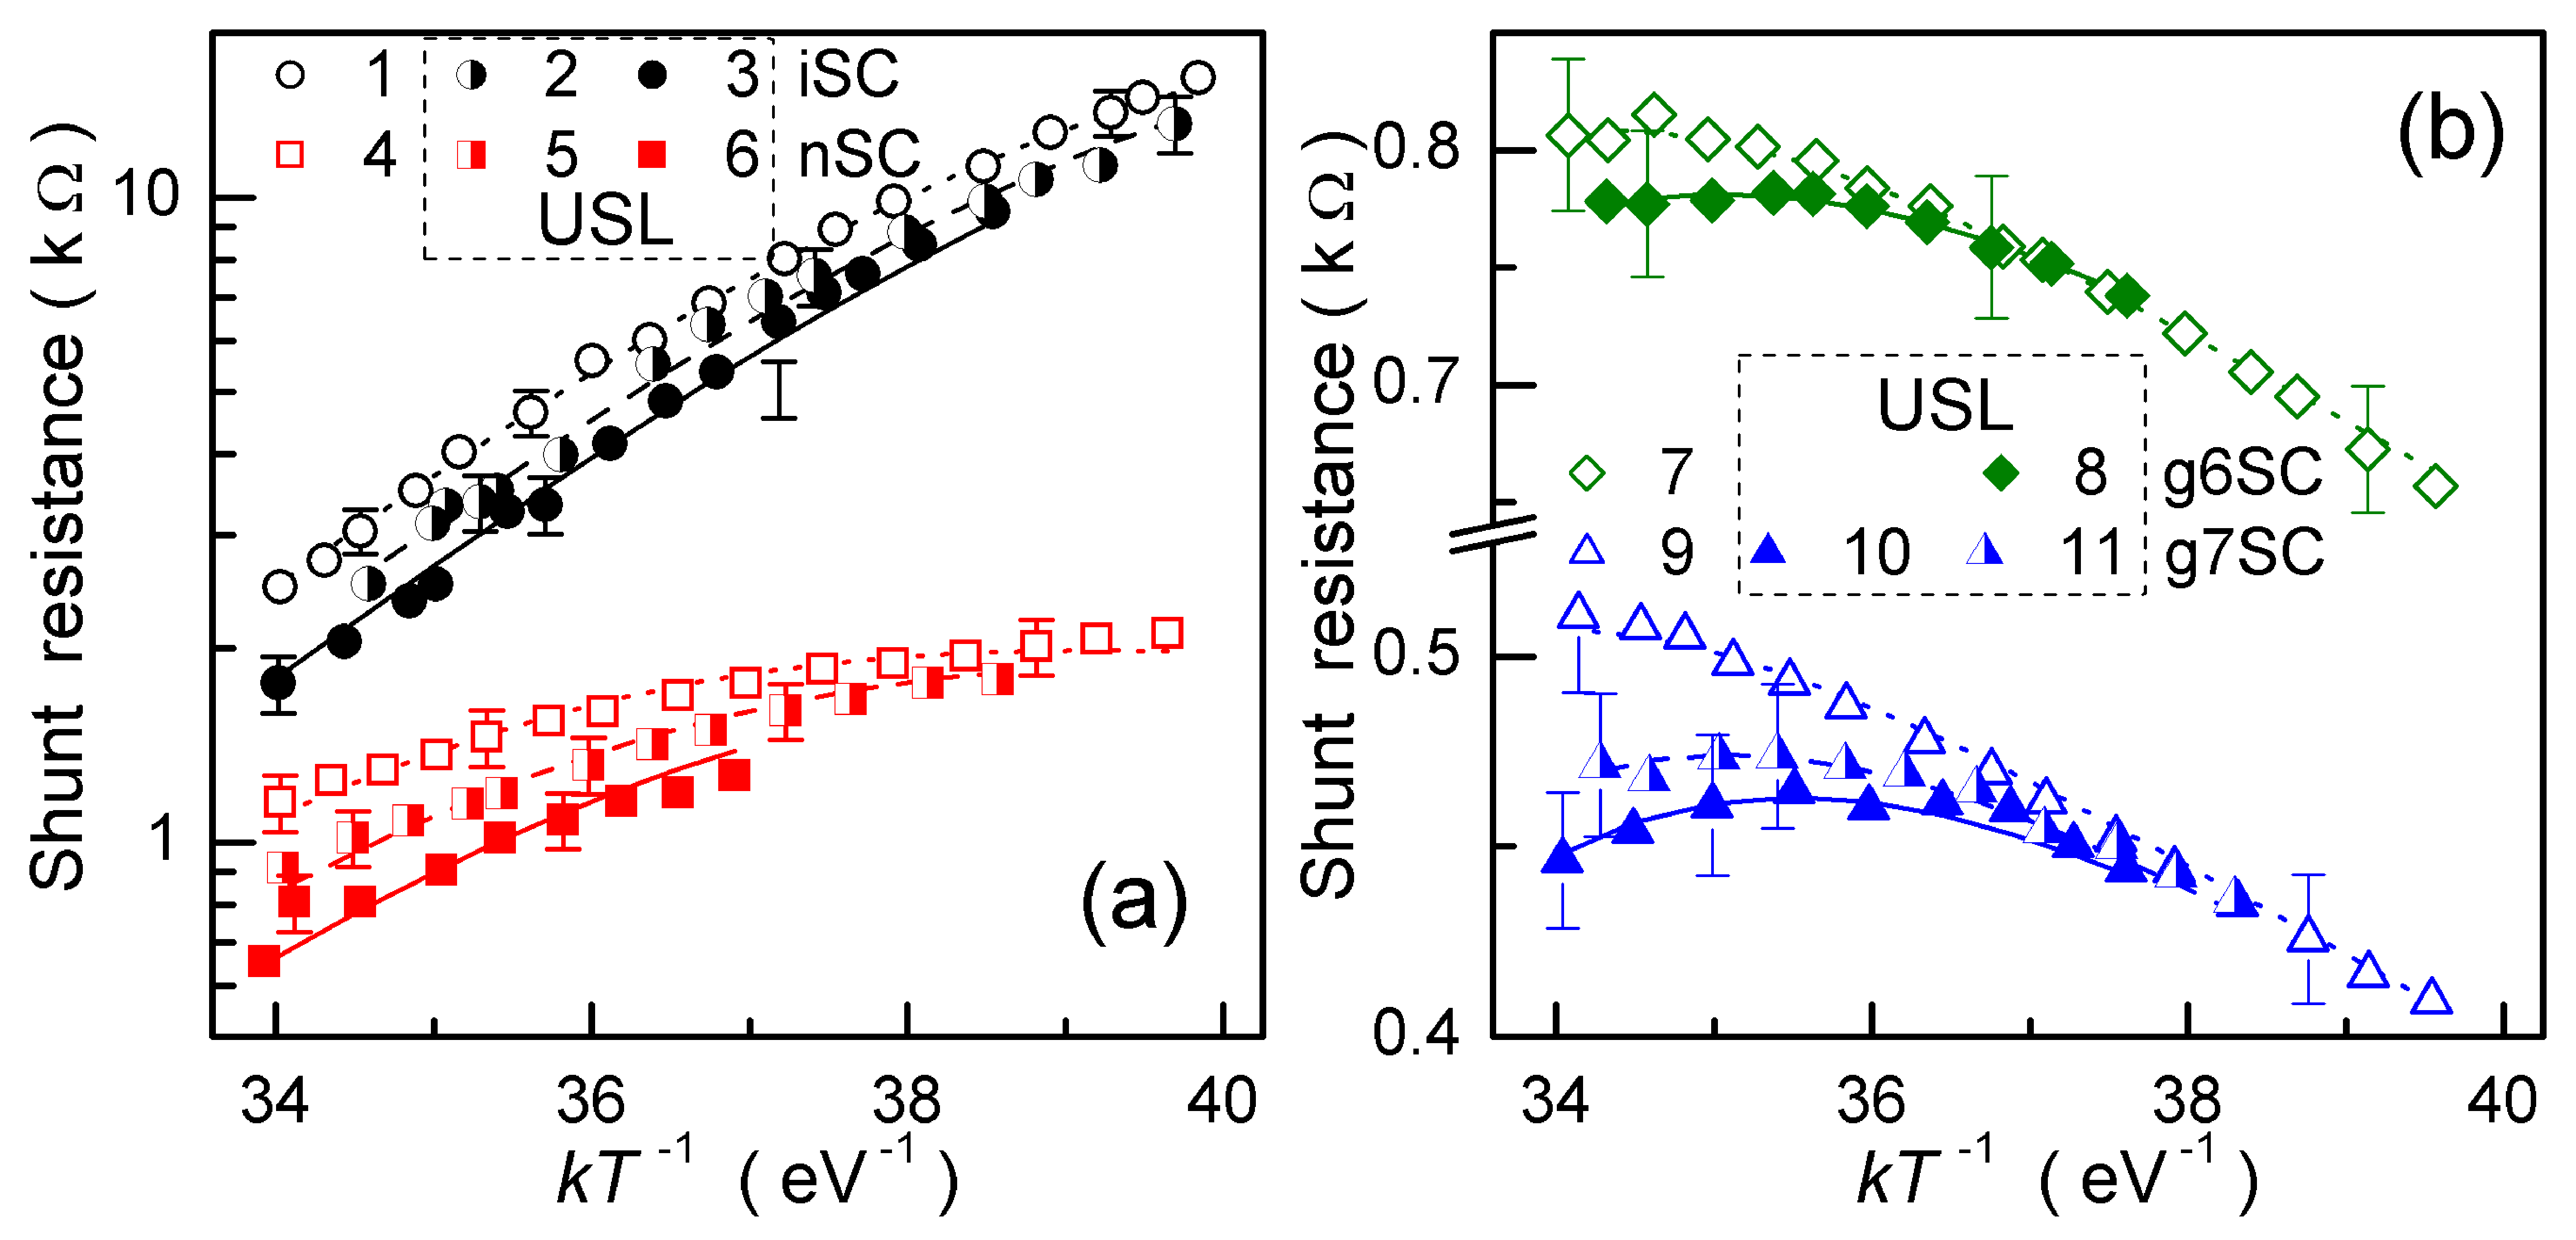
\includegraphics[width=0.7\textwidth]{fig_9ab}%
\caption{\label{fig_Rsh}
Temperature dependences of shunt resistance for non--irradiated (curves 1--3, circles),
neutron--irradiated (4--6, squares), and $\gamma$--irradiated (7--11, diamonds and triangles) samples.
The curves 1, 4, 7, and 9 (open marks) are obtained without USL,
and curves 2, 3, 5, 6, 8, 10, and 11 correspond to
Ui--1, Ui--2, Un--1, Un--2, Ug6--2, Ug7--1, and Ug7--2 respectively.
The marks are the experimental results, and the lines are the fitted curves using Eqs.~(\ref{eqRshFull})-(\ref{eqRsh}).
}%
\end{figure*}

The shunt resistance is known\cite{Rsh:Breitenstein} to occur in $p$--$n$ structure due to several non--mechanical reasons.
It can be caused by aluminum particles, macroscopic Si$_3$N$_4$ inclusions, or inversion layers at precipitates.
In the course of firing, the Al particle can penetrate into the sample creating $p^+$--doped region around it, which compensates the emitter and remains in ohmic contact with the base.
Inversion layers and Si$_3$N$_4$ inclusions occur mainly in multicrystalline silicon cells \cite{Rsh:Breitenstein} and cannot cause shunt resistance in the investigated samples.
Dislocations, however, which intersect the junction, are generally held responsible as a possible source of ohmic current.\cite{Rsh:Breitenstein,TAT:Gopal,Rsh:Baker}
In our opinion, both aluminum particles and dislocations are present in the investigated structures,
so the overall shunt resistance can be expressed as
\begin{equation}
\label{eqRshFull}
R_{sh}^{-1}=R_{sh,\mathtt{Al}}^{-1}+R_{sh,\mathtt{dis}}^{-1}\,,
\end{equation}
where
$R_{sh,\mathtt{Al}}$ and $R_{sh,\mathtt{dis}}$ deal with aluminum particles and dislocations, respectively.
The linear temperature dependence of metal particles $R_{sh,\mathtt{Al}}$ is suggested:
\begin{equation}
\label{eqRshAl}
R_{sh,\mathtt{Al}}=R_{293,\mathtt{Al}}[1+\alpha(T-293)]\,,
\end{equation}
where
$R_{293,\mathtt{Al}}$ is the shunt resistance at 293~K and
$\alpha$ is the resistance temperature coefficient.

According to the model of dislocation--induced impedance of photovoltaic detector suggested by Gopal and Gupta,\cite{Rsh:Gopal2003,Rsh:Gopal2004}
$R_{sh,\mathtt{dis}}$ can be given by:
\begin{equation}
\label{eqRsh}
R_{sh,\mathtt{dis}}=\frac{T}{\sigma_{\mathtt{dis}}}\left[\cosh\left(\frac{E_\mathtt{dis}-E_i}{kT}\right)+\cosh\left(\frac{U_s}{kT}\right)\right]\,,
\end{equation}
with
\begin{equation}
\label{eqRdis}
\sigma_{\mathtt{dis}}=\rho_{\mathtt{dis}}Aq^2A_{\mathtt{dis}}\sqrt{K_nK_p}\,N_{\mathtt{dis}}(n_p+p_p)/k\,,
\end{equation}
where
$E_{\mathtt{dis}}$ is the energy level which significantly contributes to the dislocation recombination current,
$U_s$ is the potential at the surface of the dislocation core,
$\rho_{\mathtt{dis}}$ and $A_{\mathtt{dis}}$ are the dislocation density and surface area, respectively,
$K_n$ and $K_p$ are the probabilities for electrons and holes capture by the dislocation states,
and $N_{\mathtt{dis}}$ is the density of surface states at each dislocation.
Equation~(\ref{eqRsh}) is true for the simplified case of $K_p=K_n$.

The resistance temperature coefficient was estimated from data on g7SC .
The obtained value $8.3\times10^{-3}$~K$^{-1}$ is not far from the resistance temperature coefficient of bulk Al ($4.3\times10^{-3}$~K$^{-1}$).
To fit the experimental data for $R_{sh}$, we used Eqs.~(\ref{eqRshFull})--(\ref{eqRsh}).
As the fitting parameters, $R_{293,\mathtt{Al}}$, $(E_{\mathtt{dis}}-E_i)$, $U_s$, and $\sigma_{\mathtt{dis}}$ were taken.
It has been found that the experimental data are in good agreement with the fitting curves (see Fig.~\ref{fig_Rsh}) for values $(E_{\mathtt{dis}}-E_i)=(0.46\pm0.02)$~eV and $U_s=(5\pm4)\times10^{-8}$~eV, which were independent of irradiation and USL.
The obtained value of $(E_{\mathtt{dis}}-E_i)$ corresponds to the carrier activation energy $0.10\pm0.02$~eV and
is comparable with the
activation energy of dislocation levels $0.08$~eV,
which was earlier reported\cite{disl10:Castaldini,disl10:Isakova,disl10:Yu,disl10:Kveder,disl10:Trushin}
in Cz--Si:B too.\cite{disl10:Castaldini,disl10:Isakova,disl10:Yu}


The obtained values of $R_{293,\mathtt{Al}}$ and $\sigma_{\mathtt{dis}}$ are given in Table~\ref{tabTpar}.
$R_{293,\mathtt{Al}}$ does not depend on USL and increases with the irradiation level.
In our opinion, $R_{sh,\mathtt{dis}}$ is smaller than $R_{sh,\mathtt{Al}}$ in iSC.
The irradiation facilitates the formation of vacancies as well as Al diffusion out of the electrodes.
As a consequence, the number of Al particles grow, and $R_{sh,\mathtt{Al}}$ decreases and becomes the key factor contributing to the overall shunt resistance.
Al diffuses more effectively in the samples exposed to $\gamma$ radiation due to a more uniform distribution of irradiation--induced single vacancies.

Dispersion of $\sigma_{\mathtt{dis}}$ correlates with dispersion of $\tau_n$ over the samples set.
Hence, $\sigma_{\mathtt{dis}}$ dispersion deals with wafer inhomogeneity too.
USL causes  $\sigma_{\mathtt{dis}}$ increase, relative AI changes
$\varepsilon_{\sigma\mathtt{dis}}=(\sigma_{\mathtt{dis,US}}-\sigma_{\mathtt{dis},in})/\sigma_{\mathtt{dis},in}$
are shown in Table~\ref{tabAIchange}.
In our opinion, this is caused by an $A_\mathtt{dis}$ augmentation.
Namely, the dislocation core atom displacement  is  normal to the  current direction.
As a result, the carriers are captured by dislocation levels from enlarged volume.
Therefore, the effective surface area increases and $R_{sh,\mathtt{dis}}$ decreases due to US action.


\subsection{Defect type speculation\label{DefectType}}

Lifetime killers  in boron--doped Czochralski--grown Si are boron--oxygen related (BO) defects,\cite{LIDRev,LIDRev2}
iron--boron pairs \cite{MurphyJAP2011,FeB:Vahanissi,FeB:Schmidt} (or another Fe--related trap in the $n^+p$--junctions \cite{TeimurazPSS,TeimurazJAP}),
and oxide precipitates.\cite{MurphySC2014,Oxide_Schon,MurphyJAP2011,MurphyJAP2012,Oxide:Chen,Oxide:Porrini}
The first two defects are sensitive to intensive illumination at room temperature.
To determine the major recombination center in the investigated samples, the following experimental procedure was used.
The non-irradiated sample was light soaked under illumination by a halogen lamp (2 Suns) at approximately 305~K.
The illumination time varied from 1~h to 8~h.
After illumination was terminated, the sample was exposed to room temperature in the darkness.
Over 5~h period, $I$--$V$ characteristics were measured with the interval of 10--15 min in order to determine the kinetics of the parameters at room temperature.
To estimate the permanent light--induced change, the measurements of  $I$--$V$ characteristics were performed in 48~h after illumination.
After the total time under illumination ran up to 15~h, the iSC was annealed at 200~$^\circ$C for $10$~min in darkness,  after which the measurements were carried out at room temperature.
Then, the illumination and measurements were repeated.


\begin{figure}
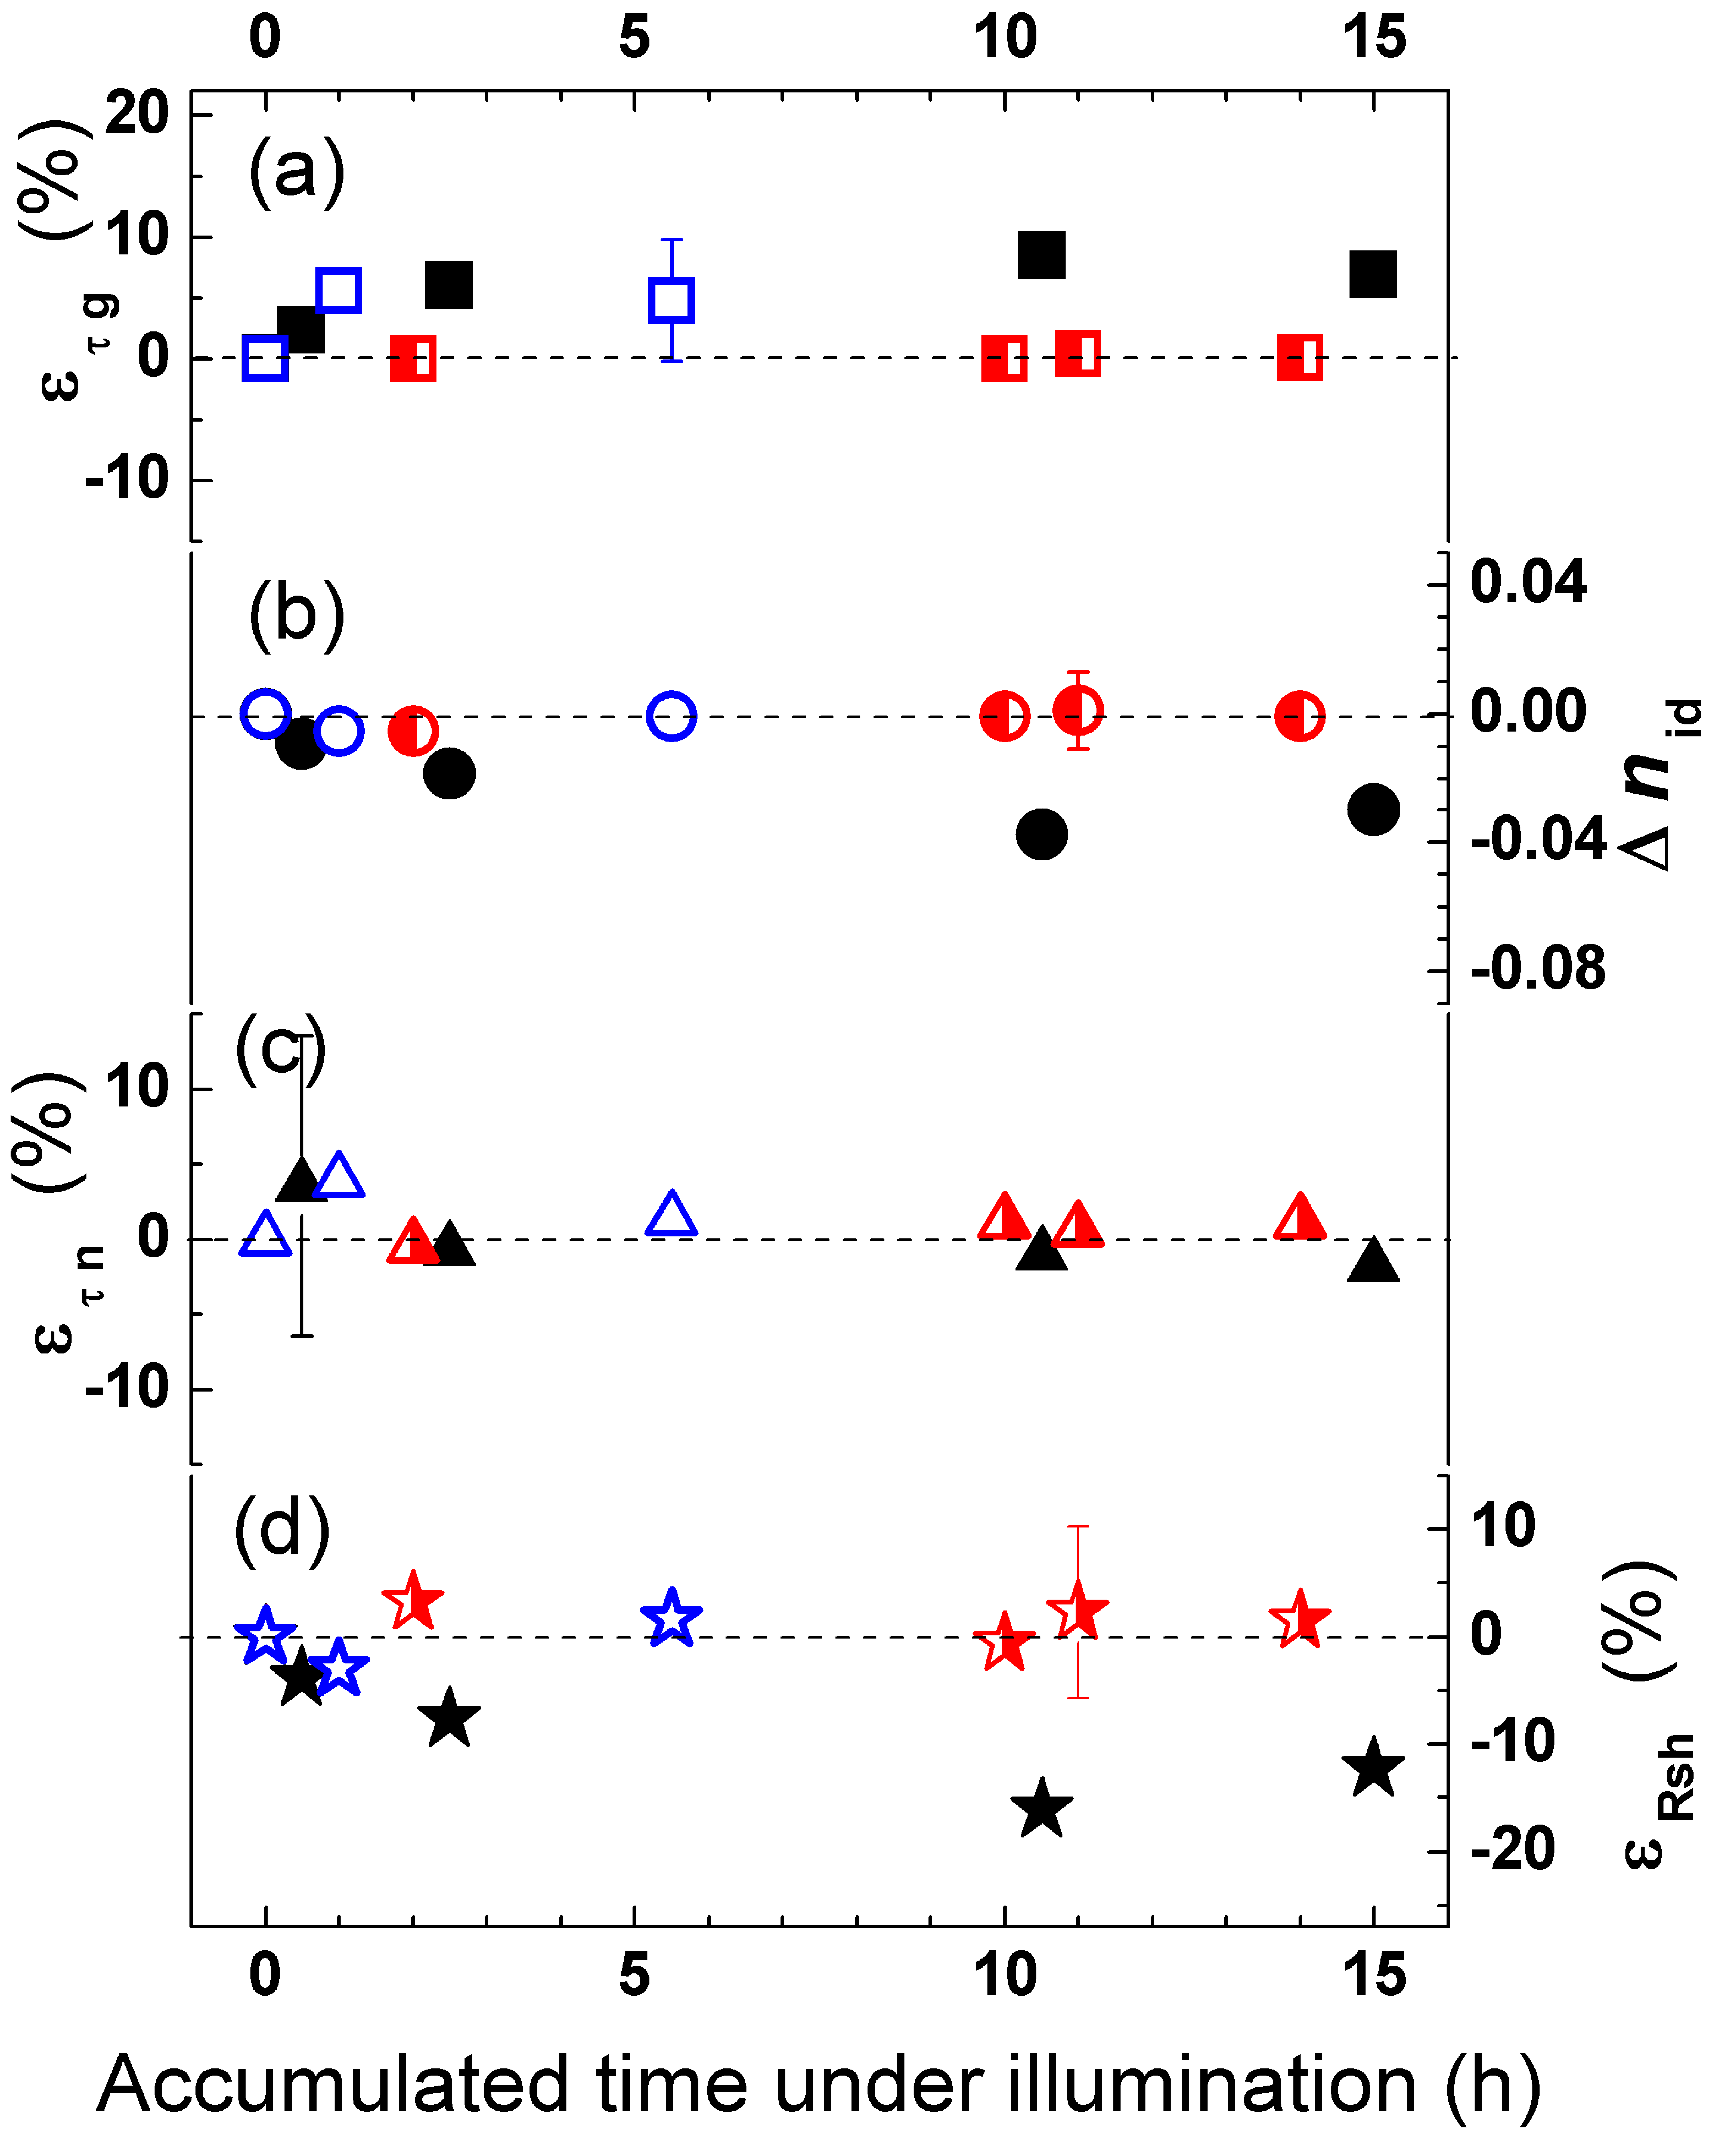
\includegraphics[width=0.46\textwidth]{fig_10}%
\caption{\label{fig_Illum}
Permanent changes of SCR lifetime [(a), squares], ideality factor [(b), circles], base lifetime [(c), triangles], and shunt resistance [(d), asterisks] versus accumulated illumination time.
Sample iSC, $T=295$~K.
Filled, semi--filled, and open marks correspond to the sample before annealing, after first $10$~min 200~$^\circ$C annealing, and after second $10$~min 200~$^\circ$C annealing, respectively.
}%
\end{figure}


Intensive light is known\cite{LIDRev,LIDRev2} to cause permanent transformation of BO defects and considerable decrease of minority--carrier lifetime (as low as 10~\% of initial value at long term illumination).
Annealing at 200~$^\circ$C for $10$~min in the darkness results in both recovery of state and readiness to light--induced degradation of BO defects.
Figure~\ref{fig_Illum} shows the changes of structure parameters in comparison with those prior to illumination.
As seen from the figure, illumination does not result in a considerable permanent change of $\tau_g$, $\tau_n$, and $n_{\mathrm{id}}$ before as well as after annealing.
Therefore, the BO influence on recombination can be neglected  in both the SCR and the base.

At the same time, the vast majority of impurity iron exists in iron--boron pairs.
Fe$_i$B$_s$ can be readily dissociated under intense illumination to release interstitial iron,
which results in lifetime changes.
In the darkness, Fe$_i$B$_s$ is repaired and Fe$_i$ concentration decreases according to \cite{MurphyJAP2011,Wijaranakula}
\begin{equation}
\label{eqFeB}
N_{Fe}(t)=(N_{Fe,\,0}-N_{Fe,\,eq})\exp\left[-\frac{t}{\tau_{\mathtt{rep}}}\right]+N_{Fe,\,eq}\,,
\end{equation}
where
$N_{Fe,\,0}$ is the concentration immediately after illumination, and $N_{Fe,\,eq}$ is the equilibrium concentration which remains for a long time after dissociation;
the characteristic time of repairing $\tau_{\mathtt{rep}}$ depends on doping level
\begin{equation}
\label{eqTrep}
\tau_{\mathtt{rep}}=770\cdot p_p^{\,-2/3}\exp\left(\frac{E_{\mathtt{D,\,Fe}}}{kT}\right)\,,
\end{equation}
$E_{\mathtt{D,\,Fe}}=0.68$~eV is the activation energy of Fe$_i$ diffusion.

\begin{figure}
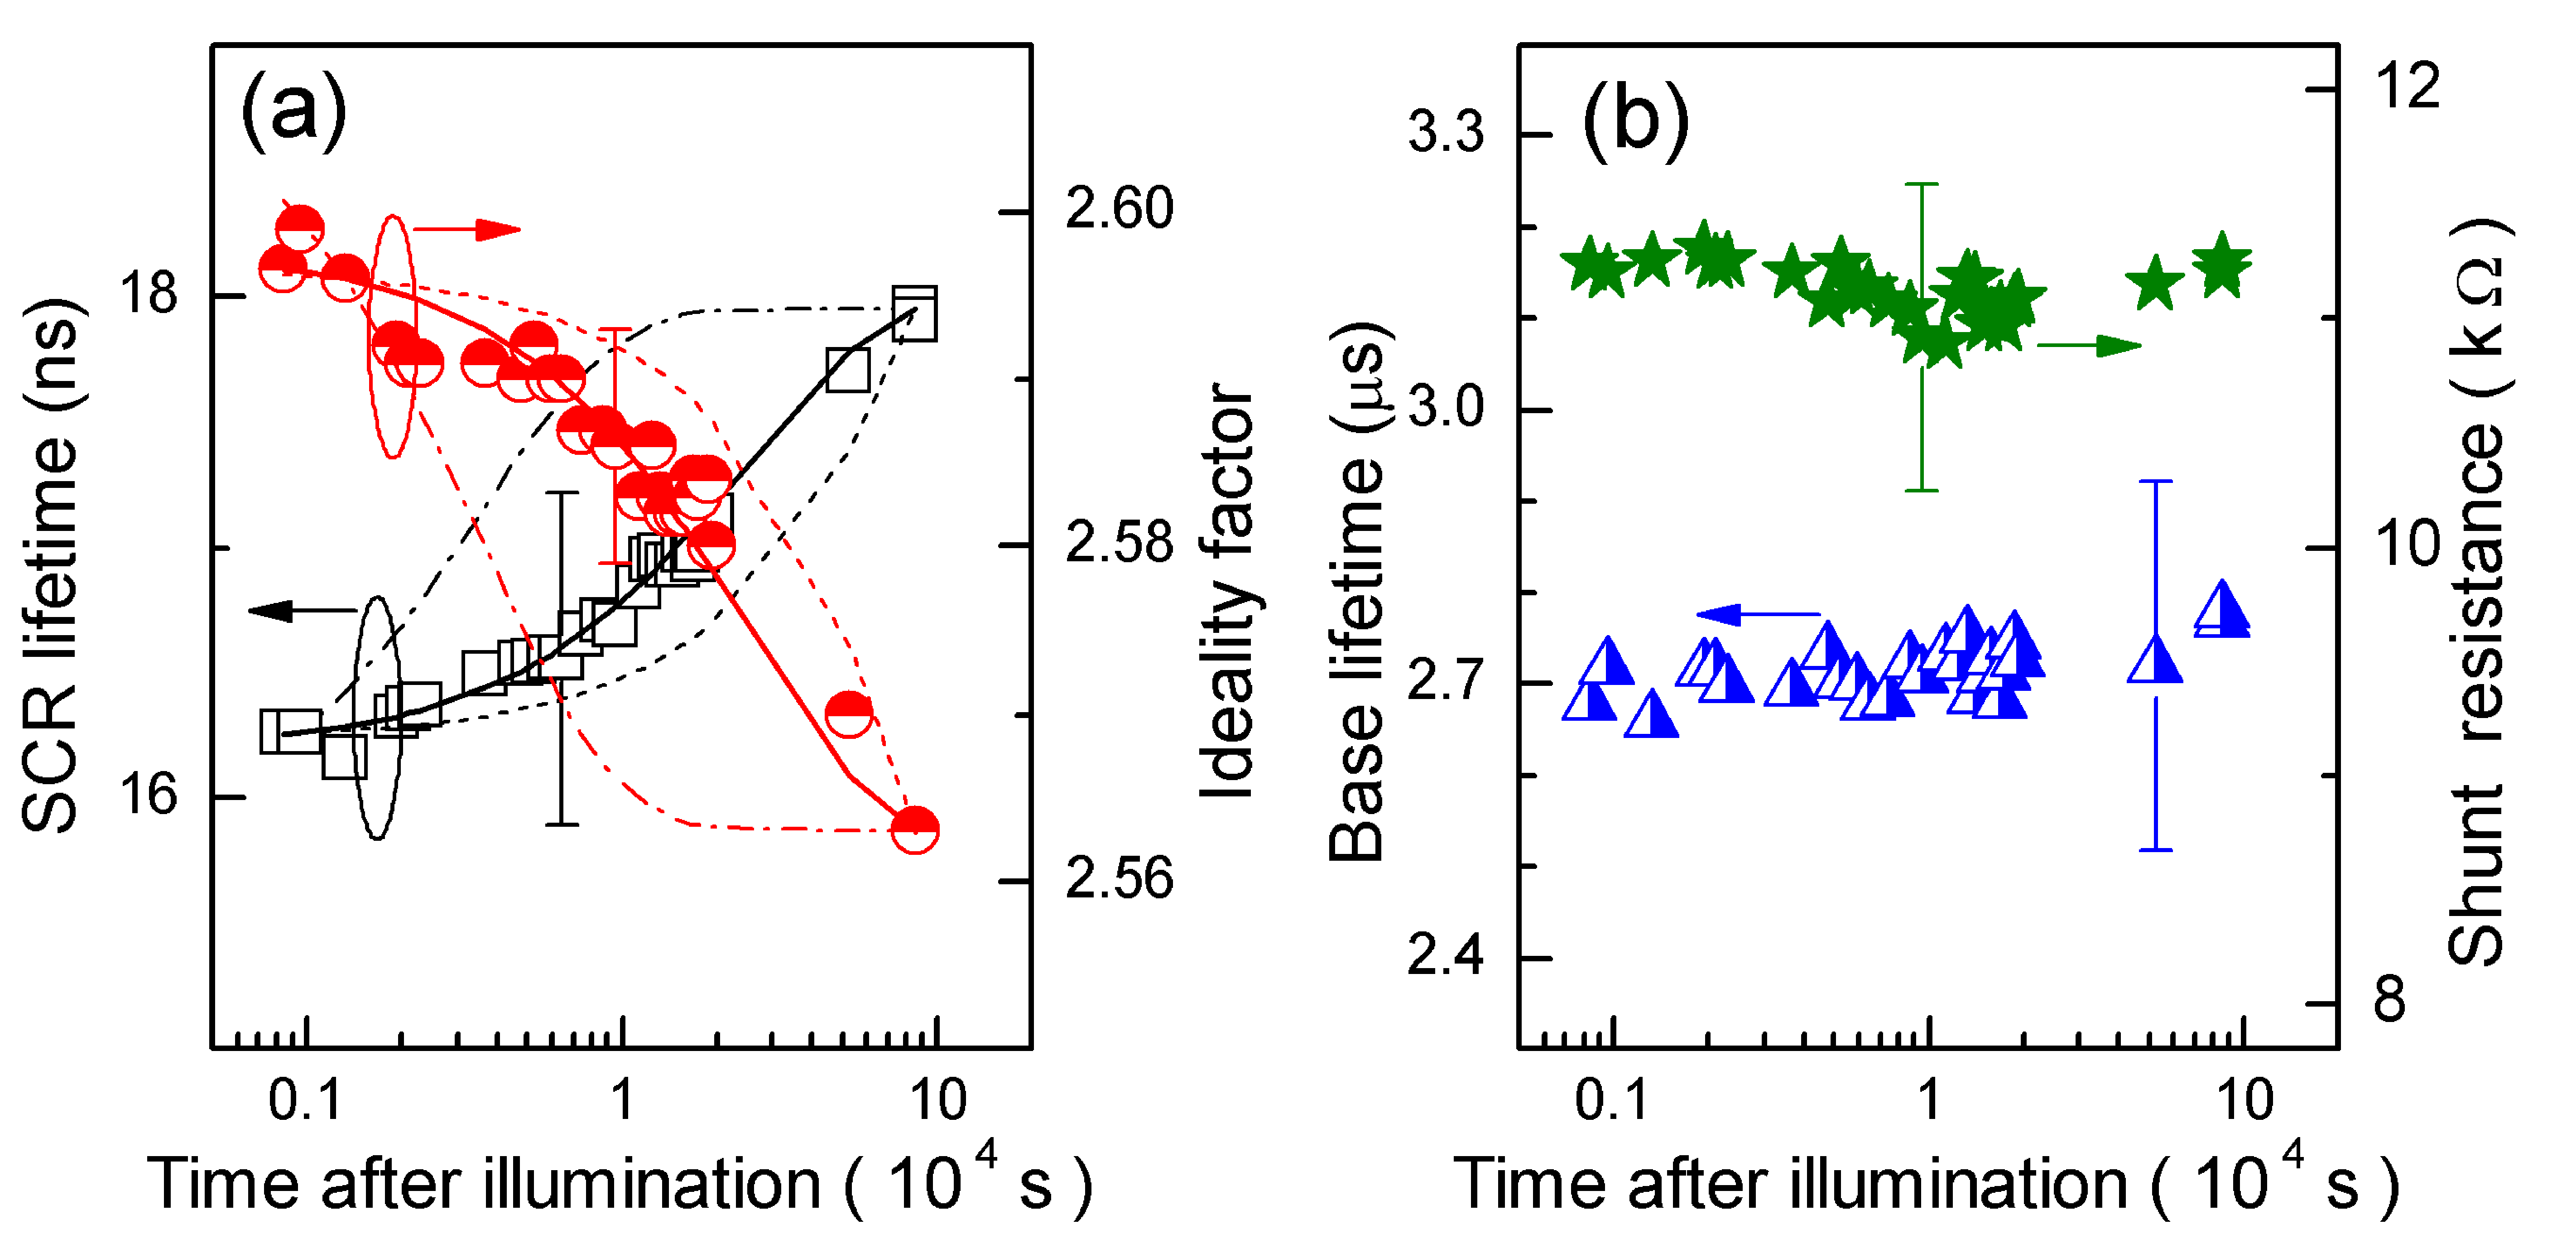
\includegraphics[width=0.47\textwidth]{fig_11ab}%
\caption{\label{fig_Time}
SCR lifetime [(a), squares, left axis], ideality factor [(a), circles, right axis], base  lifetime [(b), triangles, left axis], and shunt resistance [(b), asterisks, right axis] as a function of time since illumination stoping.
Sample iSC, $T=295$~K.
Lines are calculated by using Eqs.(\ref{eqFeB}) and (\ref{eqTrep}) and $E_{\mathtt{D,Fe}}=0.63$~eV (dashed--dotted lines), 0.68~eV (solid lines), and 0.73~eV (dashed lines).
}%
\end{figure}

It was found that $n_{\mathrm{id}}$ increased (by about 0.03) and $\tau_g$ decreased (by about 10~\%) immediately after illumination --- see Fig.~\ref{fig_Time}(a).
These changes vanished gradually.
We supposed that $\tau_g$ and $n_{\mathrm{id}}$ evolutions could be described by expressions similar to Eq.~(\ref{eqFeB}).
The obtained Eq.~(\ref{eqTrep}) was used to calculate characteristic time, and the fitting lines are presented on Fig.~\ref{fig_Time}(a).
The fittings with $E_{\mathtt{D,Fe}}=0.68$~eV are in good agreement with the experimental data.
Hence, it is evident that iron--boron pairs take part in SCR recombination.
At the same time, electron and hole CCS of Fe$_i$ are 1.7 and 0.04 times \cite{MurphyJAP2011} as much as those of Fe$_i$B$_s$.
A small $\tau_g$ alteration (by about 10~\%) caused by light is the evidence of the supporting role of iron--boron pair in SCR recombination.
Furthermore, since $\tau_n$ does not depend on illumination [see Fig.~\ref{fig_Time}(b)], Fe$_i$B$_s$ does not influence the base lifetime.

Thus, a conclusion can be made that oxide precipitates are number one agents in SCR and base recombinations.
According to Murphy \emph{et al}.\cite{MurphySC2014,MurphyJAP2012}
there exist at least two independent oxide precipitate related defects.
These defects have $\sigma_n/\sigma_p=157$ and $\sigma_p/\sigma_n=1200$, respectively,\cite{MurphyJAP2012} which is suitable for CDLR.
These facts allow us to conclude that the defect responsible for AI phenomena in iSC is mainly oxide precipitate.

In foreseeing RD type, it is worth keeping in mind doping level, oxygen concentration, and irradiation dose.
In our case (Czochralski, oxygen--rich, $\sim7\times10^{17}$~cm$^{-3}$, $p$--Si with boron concentration $\sim10^{15}$~cm$^{-3}$, and low dose),
it is expected that C$_i$O$_i$, vacancy clusters V$_n$ (divacancy V$_2$, trivacancy V$_3$, ...) and VO$_i$
are produced mainly by neutron irradiation \cite{n:long,n:gamma,Moll:PhD}
while C$_i$O$_i$ and  VO$_i$ are produced by $\gamma$--rays.\cite{gamma:Stahl,Moll:PhD,gamma:Kolk,A:Caracas}
The RD concentration $N_{t,\mathtt{RD}}$ linearly depends on the dose,
and the known introduction rate for neutron $\eta_n$ and gamma $\eta_\gamma$ irradiation in Cz--Si are shown in Table~\ref{tabDefect}.
The expected values of $N_{t,\mathtt{RD}}$ for the investigated samples are listed in Table~\ref{tabDefect} as well.


\begin{table*}
\caption{\label{tabDefect}Cited and calculated defect parameters.
}
\begin{ruledtabular}
\begin{tabular}{cccccccccc}
Defect&$\sigma_n$&$\eta_n$ (cm$^{-1}$)&$\eta_\gamma$&\multicolumn{3}{c}{$N_{t,\mathtt{RD}}$(10$^{11}$~cm$^{-3}$)}&\multicolumn{3}{c}{$\tau_{n,\mathtt{RD}}^{-1}$ (10$^4$~s$^{-1}$)}\\
&(10$^{-15}$~cm$^2$)&Reference~\onlinecite{Moll:PhD}&&nSC&g6SC&g7SC&nSC&g6SC&g7SC\\
\hline
C$_i$O$_i$&0.7 (Ref.~\onlinecite{gamma:Stahl})&1.38&6$\times$10$^5$~rad$^{-1}$cm$^{-3}$ (Ref.~\onlinecite{gamma:Stahl})&5.5&6&60&0.8--1&0.9--1.1&9--11\\
&0.9 (Ref.~\onlinecite{gamma:Kolk})&&4$\times$10$^{-4}$~cm$^{-1}$ (Ref.~\onlinecite{gamma:Kolk})&&&&&&\\
V$_2$&3 (Ref.~\onlinecite{gamma:Stahl})&1.21&3$\times$10$^4$~rad$^{-1}$cm$^{-3}$ (Ref.~\onlinecite{gamma:Stahl})&4.8&0.3&3&2.2--3.3&0.1--0.2&1--2\\
&2 (Ref.~\onlinecite{A:Brothe})&&&&&&&&\\
V$_3$&2.4 (Ref.~\onlinecite{V3:Markevich})&0.37&$\ldots$&1.5&$\ldots$&$\ldots$&0.7&$\ldots$&$\ldots$\\
VO$_i$&2.4 (Ref.~\onlinecite{A:Caracas})&0.52&7$\times$10$^5$~rad$^{-1}$cm$^{-3}$ (Ref.~\onlinecite{gamma:Stahl})&2&6--7&60--70&&&\\
&4 (Ref.~\onlinecite{A:Bleicher})&&4$\times$10$^{-4}$~cm$^{-1}$ (Ref.~\onlinecite{gamma:Kolk})&&&&&&
\end{tabular}
\end{ruledtabular}
\end{table*}

The other defects that can be created by irradiation in silicon are the I$_p$--center, bistable donor (BD), B$_i$O$_i$ and C$_i$C$_s$.
At the same time, I$_p$--center and BD are characterized by a small introduction rate.
For example, the expected\cite{n:gamma,BD:Fret} concentration of BD is only $(1-2)\times10^{10}$~cm$^{-3}$ in nSC and g7SC.
The lack of B$_i$O$_i$ in the investigated samples deals with low boron concentration \cite{SiIntDef}.
The formation of  C$_i$C$_s$ is suppressed in oxygen--rich crystal\cite{gamma:Kolk,gamma:Stahl,n:long} and, what is more,
 C$_i$C$_s$ is not an active recombination center.\cite{CiCs:Song}

The influence of RD on base lifetime could be estimated by Eq.~(\ref{eqTAUSHRsum}) taking into account the fact that
VO$_i$ is a recombination center which is not active in $p$--Si.\cite{gamma:Kolkov,IrrCzpSi:Benton,IrrCzpSi:Coffa,IrrCzpSi:Ganagona,IrrCzpSi:Vines}
The estimated $\tau_{n,\mathtt{RD}}$ for C$_i$O$_i$, V$_2$, and  V$_3$ are shown in Table~\ref{tabDefect}.
As seen from the table,  $\tau_n$ is effected mainly by C$_i$O$_i$ in $\gamma$--irradiated samples and by vacancy clusters in nSC.
It should be noted, that nSC, g6SC, g7SC sums of $\tau_{n,\mathtt{RD}}^{-1}$ are in quite good agreement with $(K_\tau\cdot\Psi)$ values.

We shall now consider $K_\mathtt{US}^\mathtt{eff}$ for non--irradiated sample assuming $M_d^\mathtt{AA}=1$ and $M_d^\mathtt{nonAA}=1$.
We shall also assume that US interactions with C$_i$O$_i$ and V$_n$ are described by $K_\mathtt{US}^\mathtt{CO}$ and $K_\mathtt{US}^\mathtt{V}$, respectively.
Then, Eq.~(\ref{eqKeff}) gives the following expression for $K_\mathtt{US}^\mathtt{eff}$
in iSC and irradiated samples:
\begin{eqnarray}
K_\mathtt{US}^\mathtt{eff}&=&K_\mathtt{US}^\mathtt{AA}\,\tau_{n,in}/\tau_{n,in}^\mathtt{AA}\,,\nonumber\\
K_\mathtt{US}^\mathtt{eff}&=&K_\mathtt{US}^\mathtt{AA}\tau_{n,in}/\tau_{n,in}^\mathtt{AA}+
                           K_\mathtt{US}^\mathtt{CO}\tau_{n,in}/\tau_{n,\mathtt{RD}}^\mathtt{CO}+
                           K_\mathtt{US}^\mathtt{V}\tau_{n,in}/\tau_{n,\mathtt{RD}}^\mathtt{V} \,.\nonumber
\end{eqnarray}
$\tau_{n,in}^\mathtt{AA}$ is the base lifetime in the sample with sole non-radiative AA defect and $K_\mathtt{US}^\mathtt{AA}$ describes ADI.


For the analysis, the following two limit cases are appropriate.
In the first one, non--AA defects are distributed uniformly across the wafer, and
AA defects define $(\tau_{n,in}^{-1}-K_\tau\cdot\Psi)$ values in different samples.
In the second one, a non--AA defect distribution is not uniform,
 and  $\tau_{n,in}^\mathtt{AA}$ is identical for iSC, nSC, g6SC, and g7SC.
However, in the first case (as well as in the case of $M_d^\mathtt{nonAA}=0$),
the experimental values of $K_\mathtt{US}^\mathtt{eff}$ lead to unreal (negative) values of $K_\mathtt{US,j}$.
In the second case, Eq.~(\ref{eqKeff}) and the data from Tables~\ref{tabTAUn} and \ref{tabDefect} give the following array equations:
\begin{eqnarray}
\mbox{iSC}:\,\,3.5&=&K_\mathtt{US}^\mathtt{AA}\cdot(\tau_{n,in}^\mathtt{AA})^{-1}\,/2.9\,,\nonumber\\
\mbox{nSC}:\,\,7.1&=&K_\mathtt{US}^\mathtt{AA}\cdot(\tau_{n,in}^\mathtt{AA})^{-1}\,/4.7+0.09\,K_\mathtt{US}^\mathtt{V}+0.02\,K_\mathtt{US}^\mathtt{CO}\,,\nonumber\\
\mbox{g6SC}:\,\,6.0&=&K_\mathtt{US}^\mathtt{AA}\cdot(\tau_{n,in}^\mathtt{AA})^{-1}\,/1.8+0.01\,K_\mathtt{US}^\mathtt{V}+0.05\,K_\mathtt{US}^\mathtt{CO}\,,\nonumber\\
\mbox{g7SC}:\,\,5.2&=&K_\mathtt{US}^\mathtt{AA}\cdot(\tau_{n,in}^\mathtt{AA})^{-1}\,/2.8+0.05\,K_\mathtt{US}^\mathtt{V}+0.35\,K_\mathtt{US}^\mathtt{CO}\,,\nonumber
\end{eqnarray}
where
$(\tau_{n,in}^\mathtt{AA})^{-1}$ in $10^4$/~s.
These equations are valid for
$K_\mathtt{US}^\mathtt{AA}\cdot(\tau_{n,in}^\mathtt{AA})^{-1}=(10\pm3)$~cm$^2$/W,
$K_\mathtt{US}^\mathtt{V}=(42\pm15)$~cm$^2$/W,
$K_\mathtt{US}^\mathtt{CO}=0$.
Since $(\tau_{n,in}^\mathtt{AA})^{-1}<1.83$, $K_\mathtt{US}^\mathtt{AA}>5$~cm$^2$/W.
Thus, the observed change in base lifetime is caused by AI modification of the same defect (most likely oxide precipitates) in
both non--irradiated and $\gamma$--irradiated samples.
This effect is enhanced by AI alteration of divacancy in neutron--irradiated samples.
In other words, C$_i$O$_i$ is the non--AA defect, whereas V$_2$ is the AA defect.


In our opinion, under US action, $\tau_g$ and $n_\mathrm{id}$ in the non--irradiated sample
depend on modification of coupled oxide precipitate related defects.
As assumed in Sec.~\ref{SCR}, in irradiated samples,
the AA radiation defects with $\Delta\Omega_d<0$ take part in CDLR.
The divacancy is a quite suitable explanation for the AI influence on $\tau_g$ and $n_\mathrm{id}$ in nSC, but in $\gamma$--irradiated samples, a bistable (or metastable) defect is expected.
A few similar defects with $\Delta\Omega_d<0$ are known in Si,
viz, VO$_2$,\cite{V2Obistable}
V$_3$,\cite{V3:Markevich}
and VO$_i$.\cite{Bistable:UFN}
VO$_2$ is formed after $300^\circ$C annealing of the irradiated crystal,
V$_3$ is not the typical defect for $\gamma-^{60}$Co exposed silicon,
while VO$_i$ is largo manum produced and can take part in CDLR around $n^+$--$p$
interface in g6SC and g7SC.
The metastable state commonly observed at low temperature is remarkable for the
large oxygen--vacancy distance and deeper energy level.\cite{Bistable:UFN}
The volume change of the entire complex is negative,
whereas for the complex component, $\Delta\Omega_d(\mbox{V})<0$ and
$\Delta\Omega_d(\mbox{O}_i)>0$.
Hence, under the assumption made, VO$_i$ is a favorable pair for AI alteration of the distance between component and therefore can be transformed into metastable configuration by USL, which
causes changes in both $T_{\mathrm{id}}$ and $E_{\tau g}$.



\section{Conclusion}
The influence of ultrasound on $I$--$V$ characteristics of non-irradiated silicon $n^+$--$p$ structures as well as silicon structures exposed to reactor neutrons or $^{60}$Co gamma radiation has been investigated experimentally.
The investigation has revealed an acoustically driven reversible decrease in the both the minority carrier lifetime and shunt resistance in the structure base.
The effect is intensified in the irradiated structures.
The analysis has shown that these effects are caused by the acoustically induced increase in the carrier capture coefficient for point or extended defects.
It has also been found that ultrasound loading leads to the reversible modification of the SCR carrier lifetime and ideality factor.
The changes are opposite in non--irradiated and irradiated structures.
The qualitative model of the observed phenomenon, which is based on the increase in the distance between coupled defects or between complex defect components due to ultrasound action, has been suggested.
It has been shown that interstitial carbon--interstitial oxygen complexes practically do not take part in acousto--defect interactions, whereas the divacancy in neutron-- exposed structures and vacancy--interstitial oxygen pairs in $\gamma$--exposed structures can be effectively modified by applying ultrasound.
Thus, ultrasound can be an effective tool for controlling silicon structure characteristics.


\bibliography{olikh}




\end{document}

